\documentclass[11pt,DIV=15]{scrreprt}


\usepackage{mathtools}
\usepackage{float}

\usepackage{etoolbox}
\newtoggle{zusammenfassung}
\toggletrue{zusammenfassung}


% Codierung
\usepackage{selinput}
\SelectInputMappings{
  adieresis={ä},
  germandbls={ß},
}
\usepackage[ngerman]{babel}
\usepackage[T1]{fontenc}
\usepackage{lmodern}

% Kopf-/Fusszeilen
\usepackage{scrlayer-scrpage}
\usepackage{lastpage}
\setkomafont{pageheadfoot}{\small\sffamily}
\pagestyle{scrheadings}
\lohead*{}
\cohead*{}
\rohead*{}
\lofoot*{XML}
\cofoot*{FS16}
\rofoot*{Seite \thepage \hspace{1pt} von \pageref{LastPage}}

% Bilder
\usepackage{graphicx}
\usepackage{subcaption}
\usepackage{color}

% Hyperlinks
\usepackage[hidelinks]{hyperref}

% Quellcode
\definecolor{keywordcolor}{rgb}{0.5,0,0.35}				% keyword color
\definecolor{stringcolor}{rgb}{0.6,0,0}					% string color
\definecolor{commentcolor}{rgb}{0.25,0.5,0.35}			% comment color
\definecolor{javadoccolor}{rgb}{0.25,0.35,0.75} 		% javadoc color

\newcommand{\code}[1]{\texttt{#1}}
\newcommand{\red}[1]{\textcolor{red}{#1}}
\newcommand{\green}[1]{\textcolor{green}{#1}}

\usepackage{listings}
\definecolor{gray}{rgb}{0.4,0.4,0.4}
\definecolor{darkblue}{rgb}{0.0,0.0,0.6}
\definecolor{cyan}{rgb}{0.0,0.6,0.6}

\lstset{
  basicstyle=\ttfamily,
  columns=fullflexible,
  showstringspaces=false,
  commentstyle=\color{gray}\upshape
}

\lstdefinelanguage{XML}
{
  morestring=[b]",
  morestring=[s]{>}{<},
  morecomment=[s]{<?}{?>},
  stringstyle=\color{black},
  identifierstyle=\color{darkblue},
  keywordstyle=\color{cyan},
  morekeywords={xmlns,version,type}% list your attributes here
}

\lstset{language=Java}
\lstloadlanguages{Java}								% language options
\lstset{
	basicstyle=\ttfamily\footnotesize,      		% fontstyle
	numbers=left,									% linenumber placement
	numberstyle=\tiny,								% linenumber fontsize
	numbersep=5pt,									% how far the line-numbers are from the code
	breaklines=true,								% print linebreaks
	commentstyle=\color{commentcolor},				% comment color
	morecomment=[s][\color{javadoccolor}]{/**}{*/}, % javadoc color
	keywordstyle=\color{keywordcolor},				% keyword color
	stringstyle=\color{stringcolor},				% string color
	showstringspaces=false,							% show spaces in a string
	frame=single,									% frame
	tabsize=4,										% tabstop
	rulecolor=\color{black},						% if not set, the frame-color may be changed on line-breaks within not-black text (e.g. comments (green here)) 
	title=\lstname,									% title is name of source file
	escapeinside={\%*}{*)},			 				% if you want to add LaTeX within your code
	inputencoding=utf8,								% encoding = utf8
	extendedchars=true,								% utf8 support 
	literate=										% utf8 support
	{á}{{\'a}}1 {é}{{\'e}}1 {í}{{\'i}}1 {ó}{{\'o}}1 {ú}{{\'u}}1
	{Á}{{\'A}}1 {É}{{\'E}}1 {Í}{{\'I}}1 {Ó}{{\'O}}1 {Ú}{{\'U}}1
	{à}{{\`a}}1 {è}{{\`e}}1 {ì}{{\`i}}1 {ò}{{\`o}}1 {ù}{{\`u}}1
	{À}{{\`A}}1 {È}{{\'E}}1 {Ì}{{\`I}}1 {Ò}{{\`O}}1 {Ù}{{\`U}}1
	{ä}{{\"a}}1 {ë}{{\"e}}1 {ï}{{\"i}}1 {ö}{{\"o}}1 {ü}{{\"u}}1
	{Ä}{{\"A}}1 {Ë}{{\"E}}1 {Ï}{{\"I}}1 {Ö}{{\"O}}1 {Ü}{{\"U}}1
	{â}{{\^a}}1 {ê}{{\^e}}1 {î}{{\^i}}1 {ô}{{\^o}}1 {û}{{\^u}}1
	{Â}{{\^A}}1 {Ê}{{\^E}}1 {Î}{{\^I}}1 {Ô}{{\^O}}1 {Û}{{\^U}}1
	{œ}{{\oe}}1 {Œ}{{\OE}}1 {æ}{{\ae}}1 {Æ}{{\AE}}1 {ß}{{\ss}}1
	{ç}{{\c c}}1 {Ç}{{\c C}}1 {ø}{{\o}}1 {å}{{\r a}}1 {Å}{{\r A}}1
	{€}{{\EUR}}1 {£}{{\pounds}}1
}

% Grafiken
\usepackage{tikz}
\usetikzlibrary{automata,matrix,chains,positioning,decorations.pathreplacing,arrows,calc}
%\usetikzlibrary{automata,arrows,positioning,calc}
\tikzset{set dim/.style={insert path={% 
   coordinate [pos=0] (tmpa) 
   coordinate [pos=1] (tmpb) 
     \pgfextra{%
      \pgfextractx{\pgf@x}{\pgfpointanchor{tmpa}{center}}
      \pgfextracty{\pgf@y}{\pgfpointanchor{tmpa}{center}}
      \pgf@xa\pgf@x %
      \pgf@ya\pgf@y %
      \pgfextractx{\pgf@x}{\pgfpointanchor{tmpb}{center}}
      \pgfextracty{\pgf@y}{\pgfpointanchor{tmpb}{center}}
      \pgf@xb\pgf@x %
      \pgf@yb\pgf@y %
      \advance\pgf@xb by -\pgf@xa 
      \advance\pgf@yb by -\pgf@ya
      }%
     }, minimum width=\pgf@xb,minimum height=\pgf@yb
     }%
  }%

% Mathematik
\usepackage{amsmath,amsfonts,amsthm, amssymb} % Math packages

% Textformatierung
\usepackage{ulem}


%\setcounter{chapter}{-1}


\begin{document}	
	
\nottoggle{zusammenfassung}{
\titlehead{Hochschule Luzern \\
	Technik \& Architektur}
\subject{Zusammenfassung}
\title{XML Technologies}
\subtitle{}
\author{Simon Neidhart \\ Kevin Wespi \\}
\date{\today}

\maketitle

}

\chapter{XML Principles}

\section{Binary vs. Text Files}

\subsection{Binary Files} 
Binärdateien sind Streams von Bits. Nur die kreierende Applikation der Datei weiss, was sie bedeuten und wie sie zu interpretieren sind.

\begin{tabular}{|p{7cm}|p{7cm}|}
\hline 
Advantage & Disadvantage \\ 
\hline 
\begin{itemize}
\item concise representation 
\item small space (e.g. hard disc)
\item less bandwidth when transported across networks 
\end{itemize} & 
\begin{itemize}
\item not readable by humans
\item only some program know how to read them
\end{itemize} \\
\hline 
\end{tabular}

\subsection{Text Files}
Textdateien benutzen Standardencodings (z.B. UTF-8).

\begin{tabular}{|p{7cm}|p{7cm}|}
\hline 
Advantage & Disadvantage \\ 
\hline 
\begin{itemize}
\item human and cross-application readable
\item easier parsing (library functions)
\end{itemize} & 
\begin{itemize}
\item  space consuming (metadata needs to be separated from content) 
\end{itemize} \\ 
\hline 
\end{tabular} 

\section{Metadaten}
Metadaten sind Information über Informationen, wie z.B. Encoding, Version, Autor, Sprache, Repräsentation (Font, Farbe), Gerät.

Metadaten müssen vom Inhalt abgegrenzt werden.

\section{SGML - Der Vorgänger von XML}
Die Vorteile von Textdateien entstehen durch das Standardcharakterencoding. Menschen wollten ebenfalls die Separierung der Metadaten standardisieren. Erster Standard entstand um 1986 mit SGML: Text and Office Systems Standard Generalized Markup Language. Das SGML-Konzept war zwar gut, aber viel zu kompliziert. HTML (erste Version war 1992) ist auch eine SGML Sprache.

\section{XML - Extensible Markup Language}
\begin{itemize}
\item 1996 als Subset von SGML von W3C publiziert
\item XML spezifiziert nur die Regeln für das Hinzufügen von Metadaten.
\item Anders als SGML spezifiziert XML \textbf{nicht}, welche Metadaten erlaubt sind.
\end{itemize}

Creators of XML: The power of metadata warrants bigger files (... terseness is not an aim ...).
Es gibt verschiedene Möglichkeiten um die Grösse der Files zu reduzieren (z.B. Komprimierung).
Das bedeutet allerdings einen Austausch gegen Lesbarkeit und "`Ease of use"'.
Warum soll man nicht komprimierte Files speichern (z.B. ZIP)? Ein Bitfehler kann die ganze Scheisse zerstören.

\subsection{Advantages of XML}
\begin{enumerate}
\item Sehr strikte, aber simple Formatierungsregeln
\begin{itemize}
\item Bietet generische Parsing-Frameworks, wie DOM \& SAX.
\item Automatische Code-Generierung à la JAXP oder WSDL.
\item Ungültige Files können zurückgewiesen werden, bevor es zu Fehlern in der Applikation kommt.
\end{itemize}
\item Recreation of corrupted files
\begin{itemize}
\item Im Gegensatz zu Binärformaten ist das Recovery von XML-Dateien relativ einfach.
\end{itemize}
\item Interoperabilität
\begin{itemize}
\item Verschiedene Parteien können einfach ein austauschbares Format definieren.
\item XSD anstatt lange Fileformatspezifikation (wie z.B. bei einem Binärfile).
\end{itemize}
\item XML ist sehr gut geeignet für Datenzentrische und Dokumentzentrische Verwendung.
\end{enumerate}


\section{Data-Centric vs Document-Centric Use of XML}
\subsection{Data-Centric Use of XML}
Datenzentrische XNL Dokumente haben viele kleine Datenitems, die einer spezifischen Struktur folgen.

Beispiel: Config File

\begin{lstlisting}
<folder name="C:">
	<folder name="Windows">
		<folder name="system32">
			<files>
				<file name="fsutil.exe" />
				<file name="ftp.exe" />
			</files>
		</folder>
	</folder>
</folder>
\end{lstlisting}

\subsection{Document-Centric Use of XML}
Diese XML-Dokumente enthalten grössere Mengen von Fliesstext ohne gross strukturierte Daten.

Beispiel: XHTML webpage

\begin{lstlisting}[language=XML]
<ul><li><strong>Computer Science Fundamentals:</strong> This is an introductory
course to computer science for students in various engineering disciplines. Topics
include programming languages and programming fundamentals in Java, computer
architectures, operating systems, elementary computer mathematics and Boolean logic,
computer science in business, cloud computing, security, a hint of artificial
intelligence, network technology and the internet, etc.</li><li><strong>Information
Security:</strong> My part of this course focusses on selected (privacy-preserving)
security protocols for electronic and internet voting, royalty cards, toll pricing,
smartcard authentication (e.g. e-banking) and quantum cryptography. The second main
topic is malware and hacking techniques including buffer overflows, identity theft
(e.g. password cracking), denial-of-service attacks, SQL injection attacks, XSS and
social engineering.</li><li><strong>Introduction to Object-Oriented Programming
</strong>: This is an introductory course to Java, object-oriented paradigms and
software design and development. It further includes some classes on elementary
algorithmics with special focus on searching and sorting procedures.</li></ul>
\end{lstlisting}

\subsection{Hybride Verwendung von XML}
Hybride XML-Dateien haben sowohl strukturierte, als auch unstrukturierte Daten.

\nottoggle{zusammenfassung}{
\section{XML Anwendungen}
\subsection{Configuration and Logging}
ANT, Visual Studio Project Files, Java Logging Framework, ...
\subsection{Webservices}
Eine exakte Definition gibt es nicht. Einige würden sogar den Aufruf auf eine einfache Website als Webservice bezeichnen. Grundsätzlich lässt sich aber sagen, dass ein Webservice sowohl einen Request akzeptiert und eine Response generiert oder zumindest einen Task ausführt. Zumindest lässt sich sagen, dass der Request oder die Response aus XML besteht.

\subsection{Unterschied RPC und SOAP}
Bei RPC sehen weder Nutzer noch Service je XML (XML wird nur für Transport verwendet).
\begin{figure}[h!]
\centering
\small
\begin{tikzpicture}[->, >=stealth', auto, semithick, node distance=2cm]
\tikzstyle{every state}=[fill=white,draw=black,thick,text=black,scale=1]
\fill [blue!20] (-4,0.5) rectangle (11.5,2.5);
\node (rect)    (C) at (4,4) [draw,thick] {Client};
\node (rect)    (S) at (2,4) [draw,thick] {Server};
\node (rect)    (M) at (3,2) [draw,thick] {Middleware};
\node[blue] at (8,1) {XML};
\path
(C) edge[left,right] node{1. Methodenaufruf mit Parametern} (M)
(M) edge[loop right] node{2. Verpacken des Aufrufs in XML File} (M)
(M)	edge[loop below] node{3. Senden zur Middleware des Servers}(M)
(M)	edge[loop left] node{4. Entpacken des XML Files}(M)
(M) edge[left,left] node{5. Methodenaufruf auf Server mit Parametern} (S);
\end{tikzpicture}
\caption{RPC Aufruf Client $\rightarrow$ Server}
\end{figure}
\\
In Listing \ref{lst:webservicerequest} ist dargestellt, wie ein Aufruf der Methode \code{MathService.Add(17,29)} in der Middleware zu einem XML verarbeitet werden könnte. Die Response des Servers könnte dazu wie in Listing \ref{lst:webserviceresponse} dargestellt aussehen.\\
\begin{minipage}{0.45\textwidth}
\begin{lstlisting}[language=XML, caption={Web Service Request}, label=lst:webservicerequest]
<methodCall> 
<methodName>MathService.Add</methodName> 
<params>
    <param>
      <value>
        <double>17</double>
      </value>
    </param>
    <param>
	 <value> 
		<double>29</double>
      </value>
    </param>
  </params>
</methodCall>
\end{lstlisting}
\end{minipage}
\hfill
\begin{minipage}{0.45\textwidth}
\begin{lstlisting}[language=XML, caption={Web Service Response}, label=lst:webserviceresponse]
<methodResponse>
  <params>
	<param>
	 <value>
        <double>46</double>
      </value>
    </param>
  </params>
</methodResponse>
\end{lstlisting}
\end{minipage}\\
Bei SOAP haben User und Service Zugriff auf ein XML File. Eine SOAP-Message hat einen sogenannten \code{<envelope>}-Tag, das einen \code{<header>} und einen \code{<body>} enthält. Der Header enthält Informationen über den Request, der Body enthält eine XML Node	. SOAP arbeitet gut mit XML-Encryption und Signaturen zusammen.\\
\begin{minipage}{0.45\textwidth}
\begin{lstlisting}[language=XML, caption={SOAP-Envelope}, label=lst:soapenvelope]
<soap:Envelope
xmlns:soap="http://www.w3.org/2003/05/soap-envelope/"
soap:encodingStyle="http://www.w3.org/2003/05/soap-encoding">

<soap:Header>
  <m:Trans xmlns:m="http://www.w3schools.com/transaction/"
  soap:mustUnderstand="1">234
  </m:Trans>
</soap:Header>

<soap:Body>
  <m:GetPrice xmlns:m="http://www.w3schools.com/prices">
    <m:Item>Apples</m:Item>
  </m:GetPrice>
</soap:Body>
</soap:Envelope>
\end{lstlisting}
\end{minipage}
\hfill
\begin{minipage}{0.45\textwidth}
\begin{lstlisting}[language=XML, caption={Extracted Message}, label=lst:soapextractedmessage] 
<GetPrice xmlns:m="http://www.w3schools.com/prices">
  <Item>Apples<Item>
 </GetPrice>
\end{lstlisting}
\end{minipage}\\

\subsection{Web Service Description Language (WSDL)}
\begin{minipage}{0.6\textwidth}
SOAP transportiert jede XML-Node, aber wie können wir wissen, wie ein SOAP-Request auszusehen hat? Dieses Problem wird durch die WSDL (eine XML-Sprache) durch zur Verfügung stellen eines Contracts zwischen dem Webservice und der Aussenwelt gelöst. Ein solcher Contract definiert, welches Format der Server erwartet und ebnenso, wie die Antwort des Servers dazu aussieht. Dafür gibt es mittlerweile Tools, der Informatiker muss sich also nicht mehr direkt mit WSDL-Dokumenten auseinandersetzen.
\end{minipage}
\hfill
\begin{minipage}{0.4\textwidth}
\centering
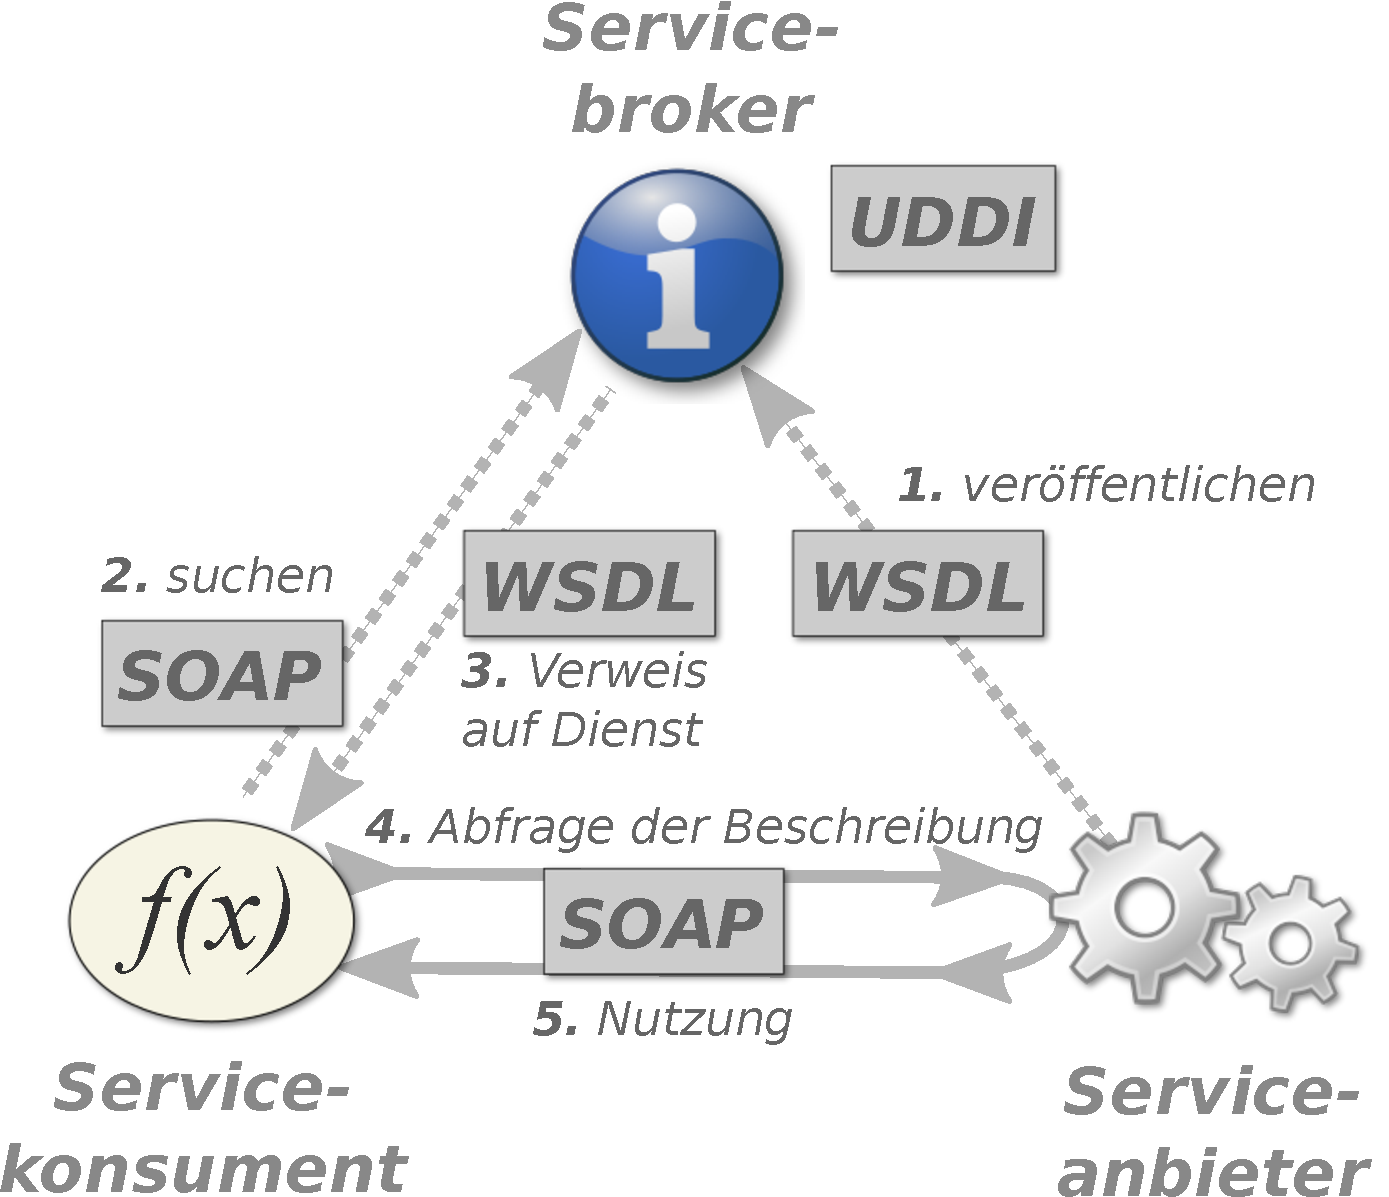
\includegraphics[width=\textwidth]{fig/Webservice.pdf}
\captionof{figure}{WSDL}
\end{minipage}\\
\subsection{UDDI - How to find Web Services in  the Wild}
Das Universal Discovery, Description and Integration (UDDI) erlaubt es, Webservices zu registrieren, damit diese von Programmierern und anderen Webservices gefunden werden können.
Das global UDDI Registry besteht aus mehreren Servern, die sich alle spiegeln: Register once, find everywhere!
Mit dem Webservice registriert man auch seine Kontaktinformationen. Eine andere Firma kann UDDI nutezn, um Businesspartner zu finden, die Dienste anbietet, die sie benötigt.

\subsection{Web Content and Type Setting}
XHTML, MATHML, SVG

\subsection{Business Interoperability}
\begin{figure}[h!]
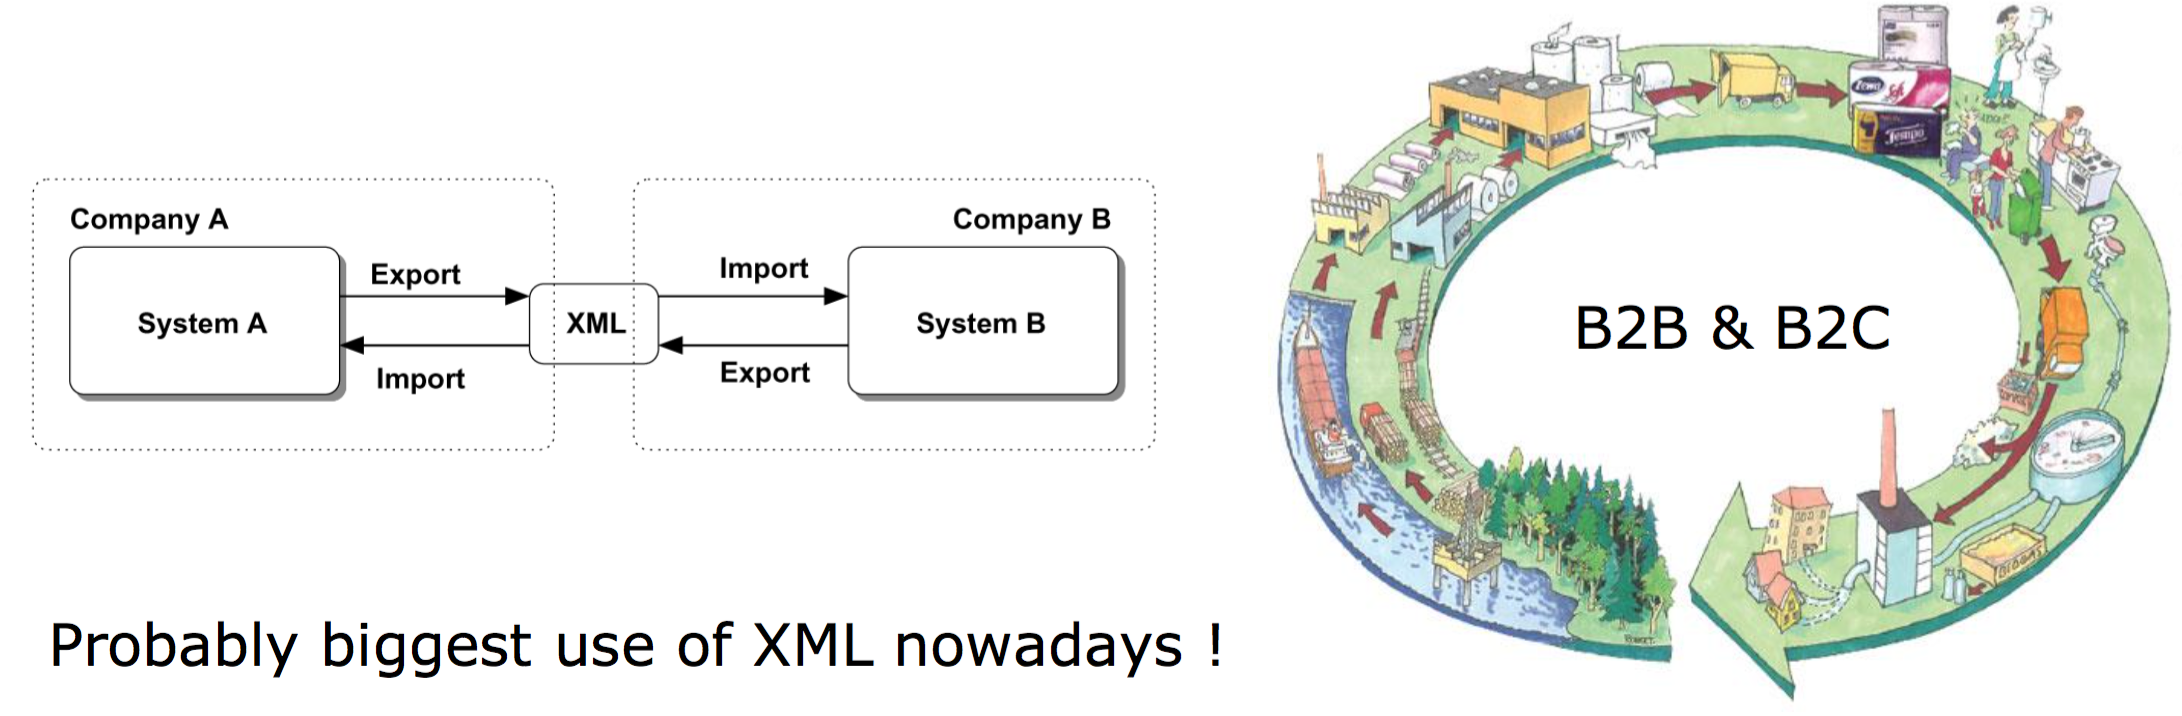
\includegraphics[width=\textwidth]{fig/Businessinteroperability.png}
\end{figure}

\subsection{Data Carrier}
Weiter in Kapitel 9
}
\nottoggle{zusammenfassung}{
\section{Intermezzo: JSON - Javascript Object Notation}
Ist ein leichtgewichtiges Datenaustauschformat. Sehr kompakt, aber immer noch gut für Menschen leserlich.

\begin{minipage}{0.45\textwidth}
\begin{lstlisting}[language=XML, caption={JSON Example}]
{"employees":[
    {"firstName":"John", "lastName":"Doe"},
    {"firstName":"Anna", "lastName":"Smith"},
    {"firstName":"Peter", "lastName":"Jones"}
]}
\end{lstlisting}
\end{minipage}
\hfill
\begin{minipage}{0.45\textwidth}
\begin{lstlisting}[language=XML, caption={XML Example}]
<employees>
    <employee>
        <firstName>John</firstName> <lastName>Doe</lastName>
    </employee>
    <employee>
        <firstName>Anna</firstName> <lastName>Smith</lastName>
    </employee>
    <employee>
        <firstName>Peter</firstName> <lastName>Jones</lastName>
    </employee>
</employees>
\end{lstlisting}
\end{minipage}\\
}
\nottoggle{zusammenfassung}{
\section{A non-religious Discussion of XML vs. JSON}
\begin{itemize}
\item JSON is more compact, easier to read and write for humans
\item JSON is a data exchange format; XML a markup language
\item JSON is better suited for data-centric use; XML is equally well suited for data-centric, document-centric and hybrid use
\item XML knows object references (id attribute)
\item XML Schema and JSON Schema* allow to define own languages.
But XML Schema knows complex data types and references
\item XPATH and XQuery extract information efficiently from deeply nested XML documents
\item XSLT enables automatic transformation of XML into different output formats (not necessarily XML)
\end{itemize}
}

\nottoggle{zusammenfassung}{
\section{CRDATA Sections}
CRDATA steht für Character Data und bedeutet, dass kein Markup verwendet wird. Es kann benutzt werden, um repetitives Escapen von Characters zu vermeiden:
\begin{lstlisting}[language=XML, caption=CRDATA]
<conversion>
	1 kilometer &lt; 1 mile
	1 pint &lt; 1 liter
	1 pound &lt; 1 kilogram 
</conversion>

<conversion>
<![CDATA[
	1 kilometer < 1 mile
	1 pint < 1 liter
	1 pound < 1 kilogram
]]>
</conversion>

\end{lstlisting}
}

\section{Processing Instructions}
Folgen gleich nach dem Prolog:\\

\code{<?xml-stylesheet type="'text/xsl"' href="'transformer.xslt"' ?>}\\

\code{<?xml-stylesheet type="'text/css"' href="'style.css"' ?>}\\\\
Sie werden von der öffnenden Applikation benutzt, um ihr Processing Instructions zu geben.

\section{Well Formed XML and Error Handling}
Ein XML ist "`wohlgeformt"' (well-formed), wenn es die obigen Regeln erfüllt. Trotzdem interpretieren Browser auch nicht-wohlgeformten HTML Code und versuchen zu interpretieren, was der Programmierer gemeint hat.

XML an sich allerdings wäre genau so strikt, wie jede andere Programmiersprache. Ein XML Prozessor wird bei in der Spezifikation als "`fatal"' definierten Errors die Ausführung stoppen (Ein Browser ist \textbf{kein} XML Prozessor, er lässt also teilweise auch richtig übles Zeug zu).

\subsection{XML Prolog}
The prolog is optional, but if it does exist then it must come first.
\begin{lstlisting}[language=XML]
<?xml version="1.0" ?>
<?xml version="1.0" encoding="ISO-8859-1" ?>
<?xml version="1.0" encoding="UTF-16" ?>
<?xml version="1.0" encoding="EUC-JP" standalone="yes" ?>
\end{lstlisting}

Version is always either 1.0 or 1.1.

XML 1.1 is not very widely implemented and is recommended for use only by those who need its unique features.)

XML allows the use of any Unicode subset. But encodings other than UTF-8 and UTF-16 will not necessarily be recognized by every parser. 

Chicken-and-Egg Problem: If an XML processor does not know the encoding, how can it read that my document uses e.g. UTF-16?

Standalone applies only to documents that specify a DTD.

\section{Equal vs Equivalent}
\begin{itemize}
\item Equal: Bit für Bit gleich
\item Equivalent: Repräsentation im Memory nach Parsing ist gleich.
\end{itemize}


\section{Control Questions A}
\begin{enumerate}
\item Name advantages and disadvantages of XML
\subitem Advantages: Check auf Wohlgeformtheit und Validierung. Über Applikationsgrenzen hinweg benutzbar, Easy to define, human readable, easy parsing, data-centric AND document-centric usage. Disadvantages: Large overhead in comparison to JSON
\item What is a markup language in general ?
\subitem Bietet eine Syntax, um Metadaten vom tatsächlichen Inhalt zu trennen.
\item Why is metadata so important that it could motivate the design and specification of a new markup language ?
\subitem It is important, because it contains Information about the Information held in the document.
\item Explain the difference between data and document-centric XML
\subitem Data-centric means that it is well structured and has many small data items (Example: DB). Document-centric means that it contains large amounts of text and there are unstructured elements (Example: XHTML)
\item Name five different application fields of XML in practice
\subitem \begin{itemize}
\item Config-Files
\item Layouting
\item Logging
\item WSDL
\item SOAP
\item Webservices
\item Data-Exchange (B2B, B2C)
\end{itemize}
\item In which field does XML apparently have the biggest success ?
\subitem Business to Business and Business to Customer
\item What are XML-RPC and SOAP, and how do they distinguish ?
\subitem Remote Procedure Call: A Middleware packs and extracts the Method Call with its parameters into XML, sends it to the server and extracts it from XML when it calls the service method. You can say that in the case of an RPC call whether the client nor the server sees an XML document (only the middleware).

In case of a SOAP-message (Called SOAP-Envelope) the server as well as the client interacts directly via XML-document.
\item Which other XML concept is used for web services ?
\subitem WSDL: Describes the functionality / ownership / location of a web service.
\end{enumerate}

\section{Control Questions B}
\begin{itemize}
\item Which information does the XML prolog contain ?
\subitem Version, Encoding and standalone
\item What are CDATA sections good for ?
\subitem They are good so that the entity reference can be left beside.
\item What is a processing instruction used for ?
\subitem To inform the browser, that some special type of formatting has to be used ("`text/css"').
\item When are two XML documents logically equivalent ?
\subitem When the representation in the memory after parsing is the same.
\item Which of the following statements are true ?
\subitem \begin{itemize}
\item Equivalent XML documents are equal.
\subitem Not mandatory.
\item Equal XML documents are equivalent.
\subitem True
\end{itemize}
\end{itemize}


\chapter{Namespaces}
\section{Why we need Namespaces}
\subsection{Namespaces}


\section{Control Questions A}
\begin{enumerate}
\item Name two* reasons why namespaces are important.\\
So that the processor knows to which Namespace a tag corresponds. Damit wir XML-Dokumente validieren (an ein Schema binden) können.
\item Explain the difference between URLs, URNs and URIs.\\
\begin{center}
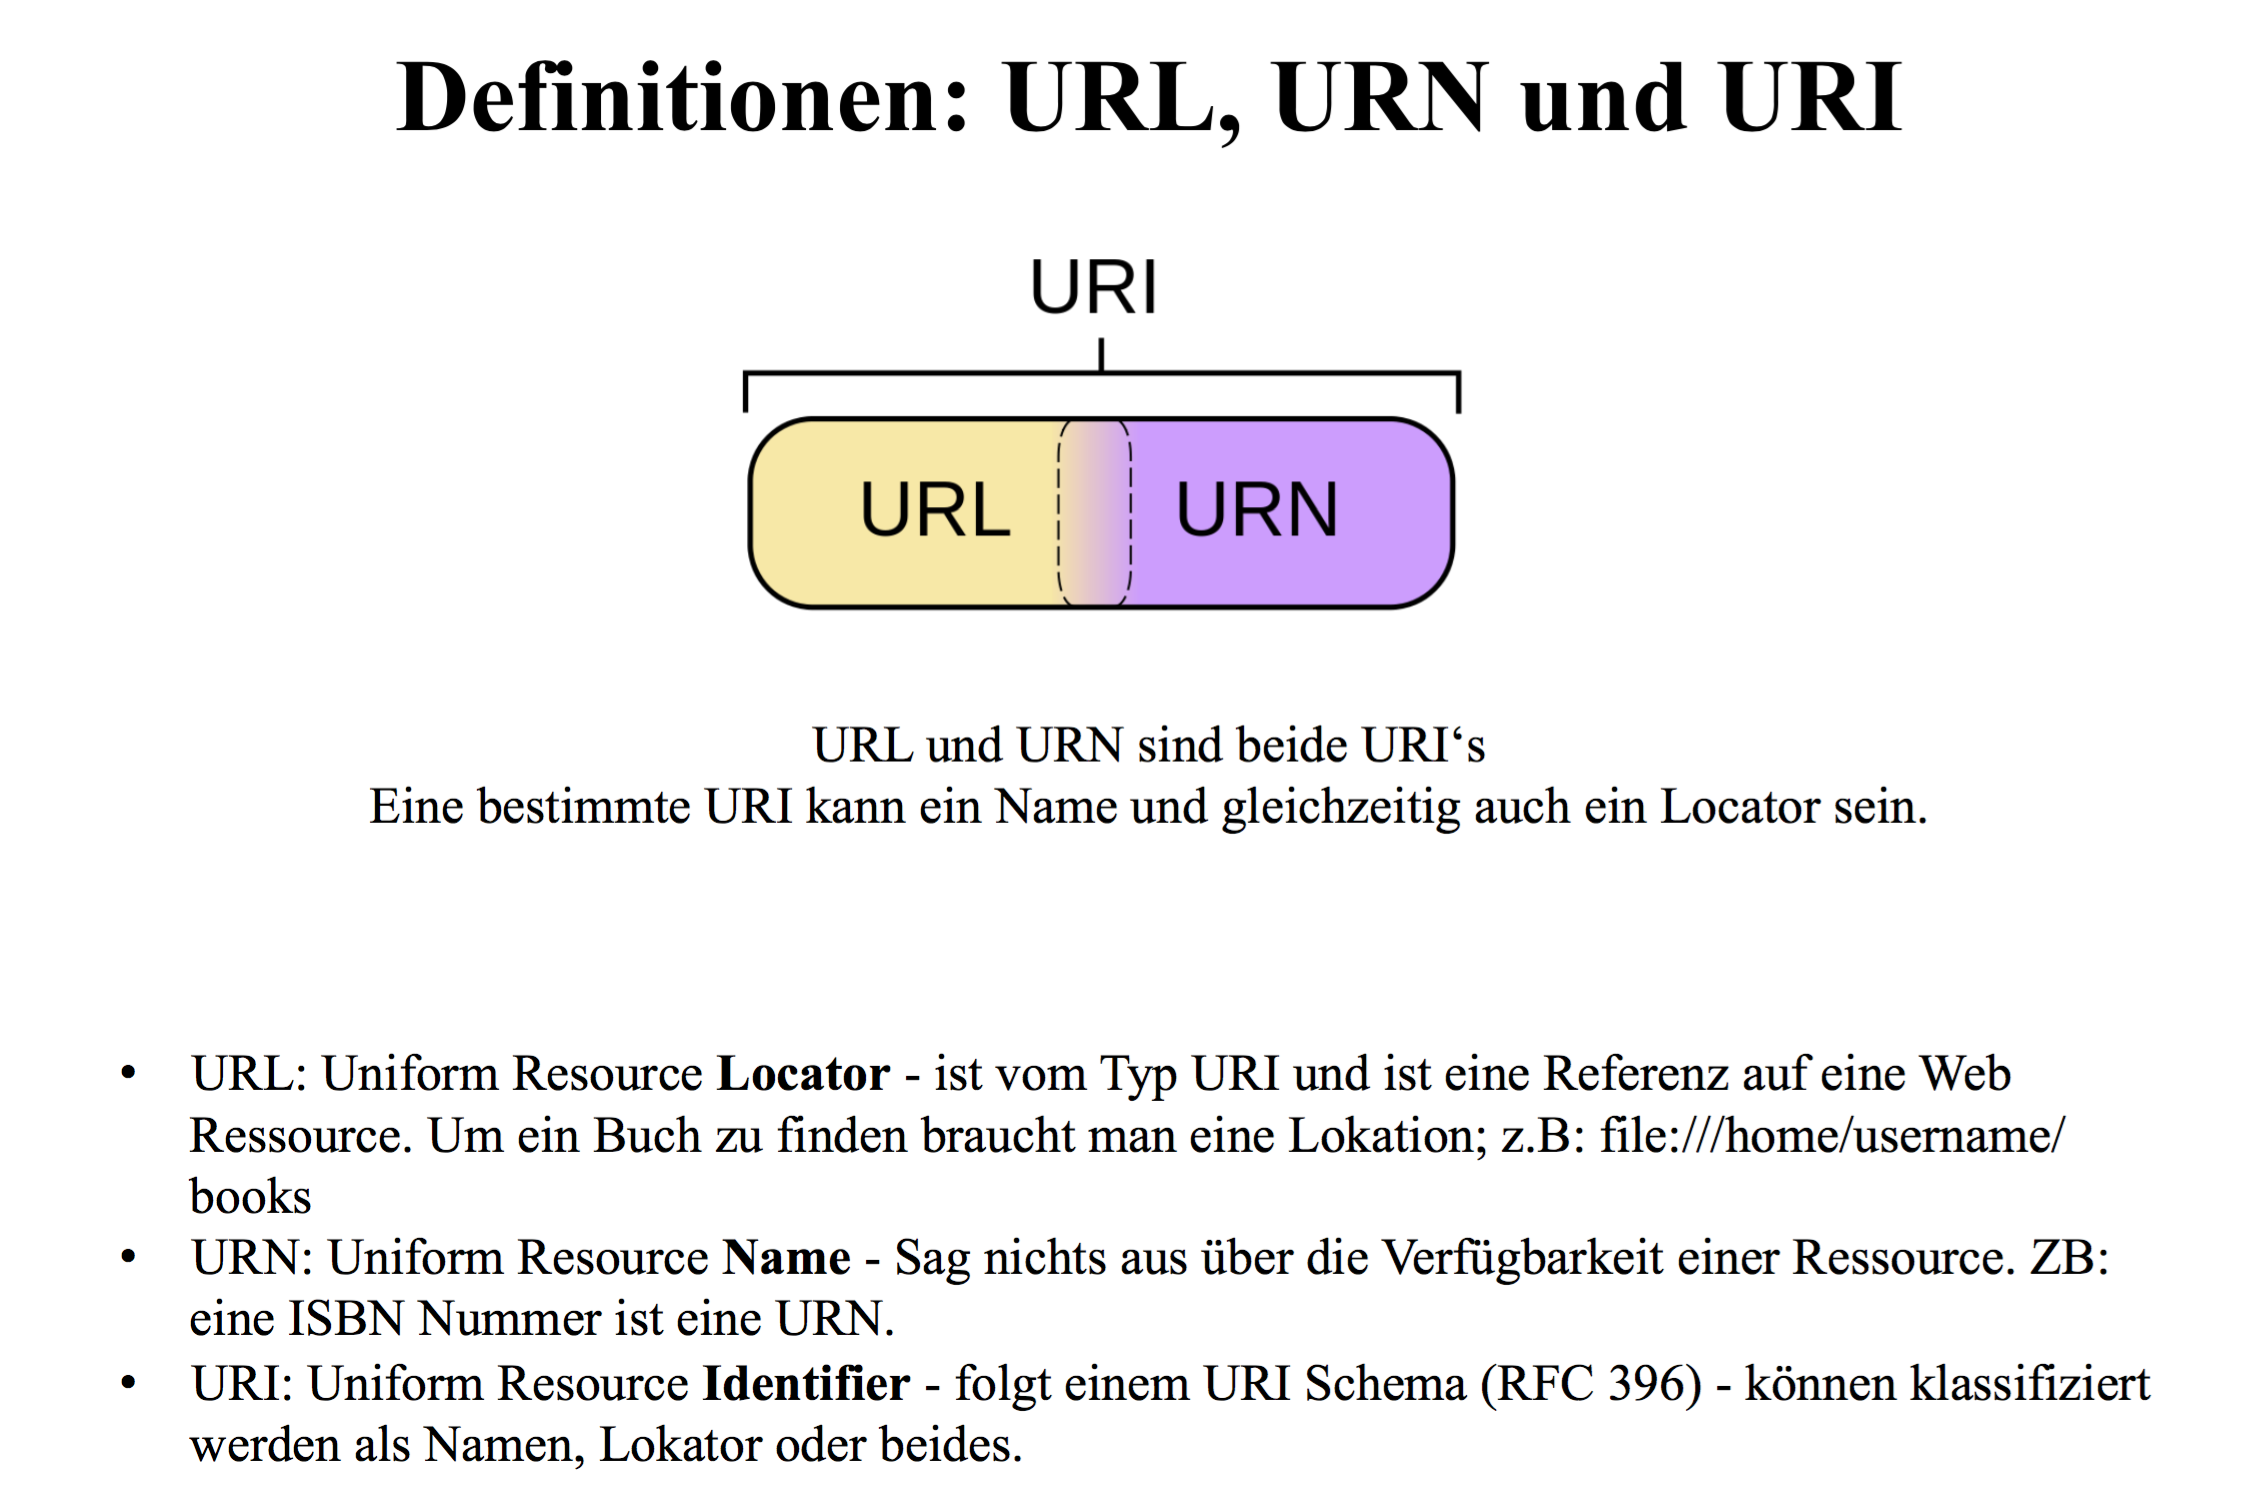
\includegraphics[width=0.7\textwidth]{fig/URI.png}
\end{center}
\item Explain the difference between a default and a prefix namespace.\\
Default Namespace inkludiert alle untergeordneten Tags in diesen Namespace, ein Prefix Namespace muss bei jedem Tag den Namespace angeben.
\item In which regard are attributes special with respect to namespaces ?\\
Attribute nehmen nicht automatisch den Namespace des Default Namespaces an, sondern müssen mit Präfix deklariert werden.
\item What is the XML namespace and why is it special ?\\
Der XML Namespace kann immer verwendet werden (ist automatisch referenziert).
\item Typical exam question on namespaces:
\begin{itemize}
\item Debug an XML document with incorrectly used namespaces
\end{itemize}
\end{enumerate}


\chapter{XPATH}
\section{XPath Axes}
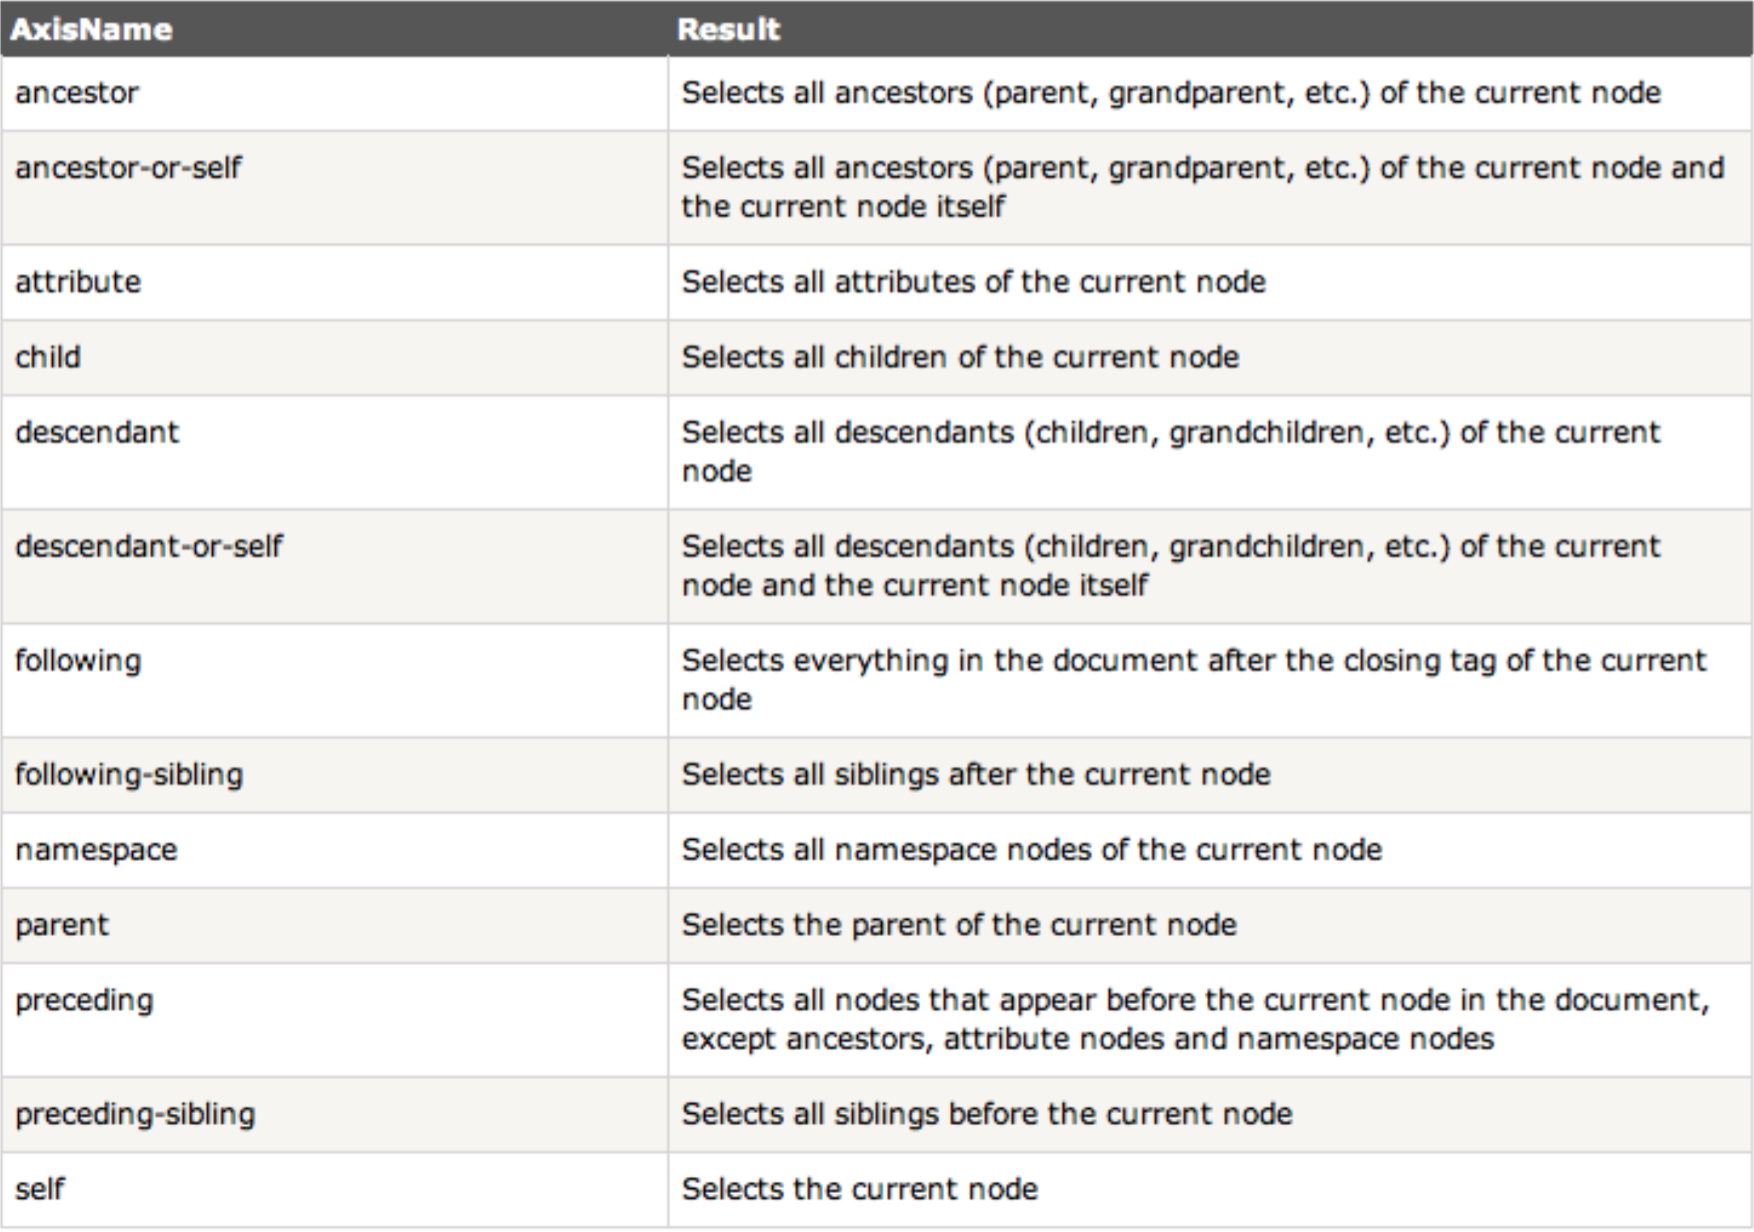
\includegraphics[width=\textwidth]{fig/XPathAxes.png}

\section{Exercises 1}
\begin{enumerate}
\item Make a prediction what the following expression returns and verify
\begin{lstlisting}[language=XML]
/descendant::title[text() = "Dr. No"]/../regie
\end{lstlisting}

\item Which number has the Bond movie with Maud Adams ?
\begin{enumerate}
\item solve the exercise with knowledge that she was a Bond Girl.
\begin{lstlisting}[language=XML]
//bond_girl[text() = "Maud Adams"]/../@number
\end{lstlisting}
\item solve it without knowing that she was a Bond Girl
\begin{lstlisting}[language=XML]
//*[text() = "Maud Adams"]/../@number
\end{lstlisting}
\end{enumerate}
\item How many times (use $count()$) did Sean Connery play Bond ?
\begin{lstlisting}[language=XML]
count(//bond[text() = "Sean Connery"])
\end{lstlisting}

\item My friends and I plan a James Bond movie night where we want to watch all movies from the very first to the very last.
How much time (use $sum()$) will this take ?
\begin{lstlisting}[language=XML]
sum(//duration)
\end{lstlisting}

\item List all movies over 120min
\begin{lstlisting}[language=XML]
//duration[text()>120]/../title
\end{lstlisting}

\item List all Bond actors without double naming (use distinct-values())
\begin{lstlisting}[language=XML]
distinct-values(//bond)
\end{lstlisting}
\end{enumerate}

\section{Exercises 2}
\begin{enumerate}
\item Formulate an XPath query that produces the following output. (<<regie>> produced <<count()>> movies)
\begin{lstlisting}[language=XML]
for $i in distinct-values(/descendant::regie) 
return concat($i, " produced ",
count(/bond_movies/movie[regie = $i]), " movies.")
\end{lstlisting}

\item Modify that it shows only regisseurs with more than one movie produced
\begin{lstlisting}[language=XML]
for $i in distinct-values(/descendant::regie) 
return if(count(/bond_movies/movie[regie = $i])>1) then
concat($i, " produced ",
count(/bond_movies/movie[regie = $i]), " movies.")
else()
\end{lstlisting}
\end{enumerate}

\section{More XPath Exercises}
Generate for the following XML:
\begin{center}
\begin{lstlisting}[language=XML]
<?xml version="1.0" ?>
<european_countries year="2012">
	<country code="CH">
		<name>Switzerland</name>
		<population>8139600</population>
		<population_under_15>14.8</population_under_15>
		<population_over_64>17.4</population_over_64>
		<life_exp_men>80.0</life_exp_men>
		<life_exp_women>84.7</life_exp_women>
	</country>
	<country code="DE">
		<name>Germany</name>
		<population>81890000</population>
		<population_under_15>13.1</population_under_15>
		<population_over_64>20.7</population_over_64>
		<life_exp_men>78.0</life_exp_men>
		<life_exp_women>82.7</life_exp_women>
	</country>
	<country code="A">
		<name>Austria</name>
		<population>8462000</population>
		<population_under_15>14.5</population_under_15>
		<population_over_64>18.1</population_over_64>
		<life_exp_men>77.1</life_exp_men>
		<life_exp_women>83.1</life_exp_women>
	</country>
	<country code="F">
		<name>France</name>
		<population>65697000</population>
		<population_under_15>18.2</population_under_15>
		<population_over_64>17.6</population_over_64>
		<life_exp_men>78.5</life_exp_men>
		<life_exp_women>84.8</life_exp_women>
	</country>
	<country code="I">
		<name>Italy</name>
		<population>60918000</population>
		<population_under_15>14.1</population_under_15>
		<population_over_64>21.2</population_over_64>
		<life_exp_men>79.3</life_exp_men>
		<life_exp_women>84.7</life_exp_women>
	</country>
	<country code="E">
		<name>Spain</name>
		<population>46218000</population>
		<population_under_15>15.4</population_under_15>
		<population_over_64>17.7</population_over_64>
		<life_exp_men>78.4</life_exp_men>
		<life_exp_women>84.6</life_exp_women>
	</country>
	<country code="GR">
		<name>Greece</name>
		<population>11280000</population>
		<population_under_15>14.6</population_under_15>
		<population_over_64>20.1</population_over_64>
		<life_exp_men>77.6</life_exp_men>
		<life_exp_women>82.9</life_exp_women>
	</country>
	<country code="NL">
		<name>Netherlands</name>
		<population>16768000</population>
		<population_under_15>17.1</population_under_15>
		<population_over_64>16.8</population_over_64>
		<life_exp_men>78.9</life_exp_men>
		<life_exp_women>83.2</life_exp_women>
	</country>
	<country code="S">
		<name>Sweden</name>
		<population>9517000</population>
		<population_under_15>16.9</population_under_15>
		<population_over_64>19.1</population_over_64>
		<life_exp_men>79.0</life_exp_men>
		<life_exp_women>83.4</life_exp_women>
	</country>
	<country code="B">
		<name>Belgium</name>
		<population>11142000</population>
		<population_under_15>17.0</population_under_15>
		<population_over_64>17.6</population_over_64>
		<life_exp_men>76.6</life_exp_men>
		<life_exp_women>83.0</life_exp_women>
	</country>
	<country code="L">
		<name>Luxembourg</name>
		<population>531000</population>
		<population_under_15>17.5</population_under_15>
		<population_over_64>14.0</population_over_64>
		<life_exp_men>76.6</life_exp_men>
		<life_exp_women>83.3</life_exp_women>
	</country>
	<country code="IS">
		<name>Iceland</name>
		<population>320000</population>
		<population_under_15>20.7</population_under_15>
		<population_over_64>12.9</population_over_64>
		<life_exp_men>78.9</life_exp_men>
		<life_exp_women>83.4</life_exp_women>
	</country>
	<country code="P">
		<name>Portugal</name>
		<population>10524000</population>
		<population_under_15>14.8</population_under_15>
		<population_over_64>19.4</population_over_64>
		<life_exp_men>75.6</life_exp_men>
		<life_exp_women>82.3</life_exp_women>
	</country>
	<country code="DK">
		<name>Denmark</name>
		<population>5590000</population>
		<population_under_15>17.6</population_under_15>
		<population_over_64>15.7</population_over_64>
		<life_exp_men>76.5</life_exp_men>
		<life_exp_women>81.2</life_exp_women>
	</country>
	<country code="N">
		<name>Norway</name>
		<population>5019000</population>
		<population_under_15>18.4</population_under_15>
		<population_over_64>15.7</population_over_64>
		<life_exp_men>77.8</life_exp_men>
		<life_exp_women>83.2</life_exp_women>
	</country>
	<country code="FIN">
		<name>Finland</name>
		<population>5414000</population>
		<population_under_15>16.4</population_under_15>
		<population_over_64>18.8</population_over_64>
		<life_exp_men>76.0</life_exp_men>
		<life_exp_women>83.2</life_exp_women>
	</country>
	<country code="IRL">
		<name>Ireland</name>
		<population>4589000</population>
		<population_under_15>21.6</population_under_15>
		<population_over_64>12.2</population_over_64>
		<life_exp_men>78.2</life_exp_men>
		<life_exp_women>82.8</life_exp_women>
	</country>
	<country code="GB">
		<name>United Kingdom</name>
		<population>63228000</population>
		<population_under_15>17.6</population_under_15>
		<population_over_64>17.2</population_over_64>
		<life_exp_men>78.2</life_exp_men>
		<life_exp_women>82.5</life_exp_women>
	</country>
</european_countries>
\end{lstlisting}
\end{center}
\begin{enumerate}
\item List all countries with population less than Switzerland
\begin{lstlisting}[language=XML]
for $i in /descendant::name
return if($i/../population/text() > //name[text() = "Switzerland"]/../population/text()) then
$i
else()
\end{lstlisting}

\item List all codes of countries with population less than Switzerland
\begin{lstlisting}[language=XML]
for $i in /descendant::name
return if($i/../population/text() > //name[text() = "Switzerland"]/../population/text()) 
then
$i/../@code
else()
\end{lstlisting}

\item List all countries whose average life expectance between men and women does not differ by more than 4.5 years
\begin{lstlisting}[language=XML]
for $i in //name 
return
if(($i/../life_exp_men - $i/../life_exp_women) < 4.5
and ($i/../life_exp_men - $i/../life_exp_women) > (-4.5))
then 
$i/../name
else ()
\end{lstlisting}

\item Find the country with the fewest people
\begin{lstlisting}[language=XML]
//population[not(. > //population)][1]/../name
\end{lstlisting}

\item List all countries with less than 1.5M people under 15 years
\begin{lstlisting}[language=XML]
for $i in //population_under_15
return 
if (($i/text() * $i/../population * 0.01)<1500000) then
$i/../name
else ()
\end{lstlisting}

\item Find all countries with at least 50% more young than old people
\begin{lstlisting}[language=XML]
\end{lstlisting}

\item $\textnormal{Dependency ratio}=\frac{\textnormal{Number of people aged 0-14 and those aged 65 and older}}{\textnormal{number of people aged 15-64}}\times 100$. Generate the following output:\\
Switzerland has dependency ratio 47.4926253687316 \\
Germany has dependency ratio 51.057401812688\\...
\begin{lstlisting}[language=XML]
\end{lstlisting}

\item Generate the following management summary:\\
Switzerland has negative trend\\
Germany has positive trend\\...
\begin{lstlisting}[language=XML]
\end{lstlisting}
\end{enumerate}

\chapter{XML Schemas}

\section{DTD vs XSD}
\begin{itemize}
\item XML Schema (XSD) is itself an XML language. DTDs (a relict from SGML times) use a different syntax.
\item DTDs do not fully support namespaces; XML Schema does.
\item XML Schema allows validation of element and attribute content against built-in or user-defined data types.
\item With XML Schemas we can more easily create complex and reusable structures and types.
\item HTML is not XML and therefore still needs a DTD. Other than that I believe that DTDs are dying out.
\end{itemize}

\begin{lstlisting}[language=XML, caption={DTD Example}]
<!DOCTYPE NEWSPAPER [
<!ELEMENT NEWSPAPER (ARTICLE+)> <!ELEMENT ARTICLE (HEADLINE, BYLINE, LEAD, BODY, NOTES)> <!ELEMENT HEADLINE (#PCDATA)> <!ELEMENT BYLINE (#PCDATA)> <!ELEMENT LEAD (#PCDATA)> <!ELEMENT BODY
(#PCDATA)> <!ELEMENT NOTES (#PCDATA)>
<!ATTLIST ARTICLE AUTHOR CDATA #REQUIRED>
<!ATTLIST ARTICLE EDITOR CDATA #IMPLIED> <!ATTLIST ARTICLE DATE CDATA #IMPLIED> <!ATTLIST ARTICLE EDITION CDATA #IMPLIED> <!ENTITY NEWSPAPER "Vervet Logic Times"> <!ENTITY PUBLISHER "Vervet Logic Press"> <!ENTITY COPYRIGHT "Copyright 1998 Vervet Logic Press">]>
\end{lstlisting}

\section{Three good Reasons for XML Schemas}
Regel: \red{\textbf{Wir lesen niemals XML Dokumente ein, ohne sie zu validieren!}}
\begin{enumerate}
\item An XML processing application can validate an input file against a Schema using a standard parser. This directly separates out incorrect files. Syntax checking of input files reduces to typing 3 lines of code. This is cheap, fast and produces less software bugs.
\item If you need to specify a new data exchange format with your business partners, write an XML Schema. This provides specification, documentation and validator at once.
\item Object-oriented programming languages such as Java or C\# directly allow to construct type hierarchies from XML Schemas. The same works with XML databases.
\end{enumerate}

\section{Validating XML Files against XML Schemas}
\begin{itemize}
\item If an XML document adheres an XML Schema, it is called an instance of this Schema.
\item It is possible to directly embed a Schema definition into an XML document (e.g. if the document will remain the only instance), but most of the time Schemas are in separate files.
\item There are different ways of how to validate an XML document:
\begin{enumerate}
\item Online Schema Validator, e.g. \href{http://www.corefiling.com/opensource/schemaValidate.html}{http://www.corefiling.com/opensource/schemaValidate.html} 
\item IDEs such as NetBeans have built-in validators
\item Use a parser in your favourite programming language
\end{enumerate}
\end{itemize}

\section{Exercise: Validation}

\section{XML Namespaces vs Java Packages}
\begin{enumerate}
\item XML Schemas define new XML languages or vocabularies comparable to e.g. packages in Java defining new API
\item If a class belongs to a package in Java, then this package is declared in the source code and must be imported for usage
\item Putting a class into a package in Java is not mandatory.
Likewise, putting a vocabulary into a namespace is not mandatory.
\item In the same way, if some vocabulary is part of a namespace, this namespace must be declared in the source code (XML Schema) and imported for usage (XML document)
\item A namespace assigned to a Schema is called target namespace
\end{enumerate}

\section{Example: Target Namesapce for SVG}
\begin{itemize}
\item We already saw that the namespace for SVG is
http://www.w3.org/2000/svg
This namespace is set inside the XML Schema for SVG as target namespace, check yourself:
http://www.w3.org/TR/2002/WD-SVG11-20020108/SVG.xsd
\item By the way, this is how a browser identifies SVG code and applies language specific rendering instead of a default action.
\item Most browsers have a built-in, hard-coded list of namespaces with specialized rendering, e.g. for XHTML, SVG, MathML, RSS, ...
\end{itemize}

\section{Do I need a target namesapce?}

\begin{itemize}
\item No, just refer in your XML document to an XML schema, and your code can be validated. In fact, we will do without target namespaces for most of our simple examples
\item Sometimes your XML Schema is distributed over multiple files. Then, using a target namespace, you can signal that all this vocabulary belongs to the same language.
\item If you want to combine several vocabularies in the same document (e.g. mix bond movies with country information) there can be at most one vocabulary without a target namespace.
\item Web languages like XHTML, SVG and MathML are often combined in the same document. Fortunately, they all have target namespaces.
\end{itemize}


\section{Binding without Target Namespace 1}
If the XML Schema does not define a target namespace for its vocabulary, the binding works as follows:
\begin{lstlisting}[language=XML, caption={Binding without Target Namespace 1}]
<european_countries 
	xmlns:xsi="http://www.w3.org/2001/XMLSchema-instance"
	xsi:noNamespaceSchemaLocation="countries_without_targetns.xsd"
	year="1999">
	<country>
		<name>Switzerland</name> <population>7124000</population>
		<population_under_15>17.5</population_under_15> 
		<population_over_64>15.2</population_over_64> 
		<life_exp_men>76.5</life_exp_men> <life_exp_women>82.5</life_exp_women>
	</country> ...
</european_countries>
\end{lstlisting}

\section{Binding without Target Namespace 2}
\begin{itemize}
\item The attribute value is the path or URL to the XML Schema file. \item This just points at the definition of the vocabulary and imports
all definitions from the referenced Schema.
\item The attribute noNamespaceSchemaLocation for binding an XML file to a Schema without target namespace belongs to the XML Schema language, i.e. it is part of the target namespace
http://www.w3.org/2001/XMLSchema-instance
Therefore we must import this namespace as well.
\end{itemize}

\section{Binding with Target Namespace 1}
If the XML Schema is supposed to define the target namespace \red{http://www.marcpouly.ch/countries} for its vocabulary,
the binding works as follows:
\begin{lstlisting}[language=XML, caption={Binding with Target Namespace 1}]
<european_countries 
	year="1999" 
	xmlns="http://www.marcpouly.ch/countries" 
	xmlns:xsi="http://www.w3.org/2001/XMLSchema-instance"
	xsi:schemaLocation="http://www.marcpouly.ch/countries countries_with_targetns.xsd">
	<country>
		<name>Switzerland</name> 
		<population>7124000</population> 
		<population_under_15>17.5</population_under_15> 
		<population_over_64>15.2</population_over_64> 
		<life_exp_men>76.5</life_exp_men> 
		<life_exp_women>82.5</life_exp_women>
	</country> ...
</european_countries>
\end{lstlisting}

\section{Binding with Target Namespace 2}
\begin{itemize}
\item The attribute schemaLocation for binding an XML file to a Schema with target namespace belongs to the XML Schema namespace.
\item The attribute value now is a list of namespace-location pairs separated by whitespace. The location specifies where the Schema can be found and which target namespace belongs to which Schema.
\item This imports everything that belongs to the target namespace http://www.marcpouly.ch/countries from the given XSD file.
\item We further declare http://www.marcpouly.ch/countries as default namespace because the majority of the used elements belong to this namespace (we could also use a prefix of course).
\end{itemize}
\begin{lstlisting}[language=XML, caption={Binding with Target Namespace 2}]
<european_countries 
	year="1999" 
	xmlns="http://www.marcpouly.ch/countries" 
	xmlns:xsi="http://www.w3.org/2001/XMLSchema-instance"
	xsi:schemaLocation="http://www.marcpouly.ch/countries 
	countries_with_targetns.xsd">
	<country>
		<name>Switzerland</name> 
		<population>7124000</population> 
		<population_under_15>17.5</population_under_15> 
		<population_over_64>15.2</population_over_64> 
		<life_exp_men>76.5</life_exp_men> 
		<life_exp_women>82.5</life_exp_women>
	</country> ...
</european_countries>
\end{lstlisting}

\section{XML Schema Skeleton without Target Namespace}
\begin{lstlisting}[language=XML, caption={XML Schema Skeleton without Target Namespace}]
<?xml version="1.0"?>
<xs:schema xmlns:xs="http://www.w3.org/2001/XMLSchema">
	<!-- Schema content --> 
</xs:schema>
\end{lstlisting}
\begin{itemize}
\item Because we want to use the XML Schema language we must declare the XML Schema namespace.
\item I strongly recommend to always use a prefix for the XML Schema namespace. As you define your own language elements in a Schema, parsers must be able to distinguish the two languages. We will illustrate the problems occurring without prefix later.
\end{itemize}

\section{Skeleton Extension for Target Namespace}
\begin{lstlisting}[language=XML, caption={Skeleton Extension for Target Namespace}]
<xs:schema xmlns:xs="http://www.w3.org/2001/XMLSchema"
	xmlns="http://www.marcpouly.ch/countries"
	targetNamespace="http://www.marcpouly.ch/countries" 
	elementFormDefault="qualified">
	<!-- Schema content --> 
</xs:schema>
\end{lstlisting}
\begin{itemize}
\item We further define the target namespace using the XML Schema attribute targetNamespace and also set this namespace as default
namespace for the XML Schema (we could also use a prefix).
\item We qualify all elements with elementFormDefault="qualified" in order to automatically put all elements into the target namespace (see next slide).
\end{itemize}

\section{Qualified Elements and Attributes}
\begin{itemize}
\item An element or attribute is called qualified if it belongs to a namespace.
\item By adding elementFormDefault="'qualified"' we signal that by default
all elements belong to the target namespace. The default value of this attribute is unqualified.
\item By adding \code{attributeFormDefault="'qualified"'} (default is unqualified) we would signal that attributes can be combined with elements from other languages, e.g. noNamespaceSchemaLocation from the XML Schema namespace is used inside \code{<european\_countries>}.
\item We will talk about this later again and also illustrate that in such cases we cannot work with default namespaces in instance documents anymore. Instead, we must give a prefix to every qualified attribute.
\end{itemize}

\section{Simple Elements}
\begin{lstlisting}[language=XML, caption={Simple Elements}]
<xs:element name="name" type="xs:string"/>
<xs:element name="population" type="xs:positiveInteger"/>
<xs:element name="life_exp_women" type="xs:decimal"/>
\end{lstlisting}
\begin{itemize}
\item These elements are atomic because they do not contain sub\item elements. Their content is an XML Schema simple data type.
\item Note the use of the namespace prefix here. Because <element> is prefixed, the parser can deduce that the attributes are those of
this element. However, this does not hold for the attribute values. Therefore, the simple data types has to be prefixed too.
\end{itemize}

\section{Simple Data Types}
\begin{figure}[h!]
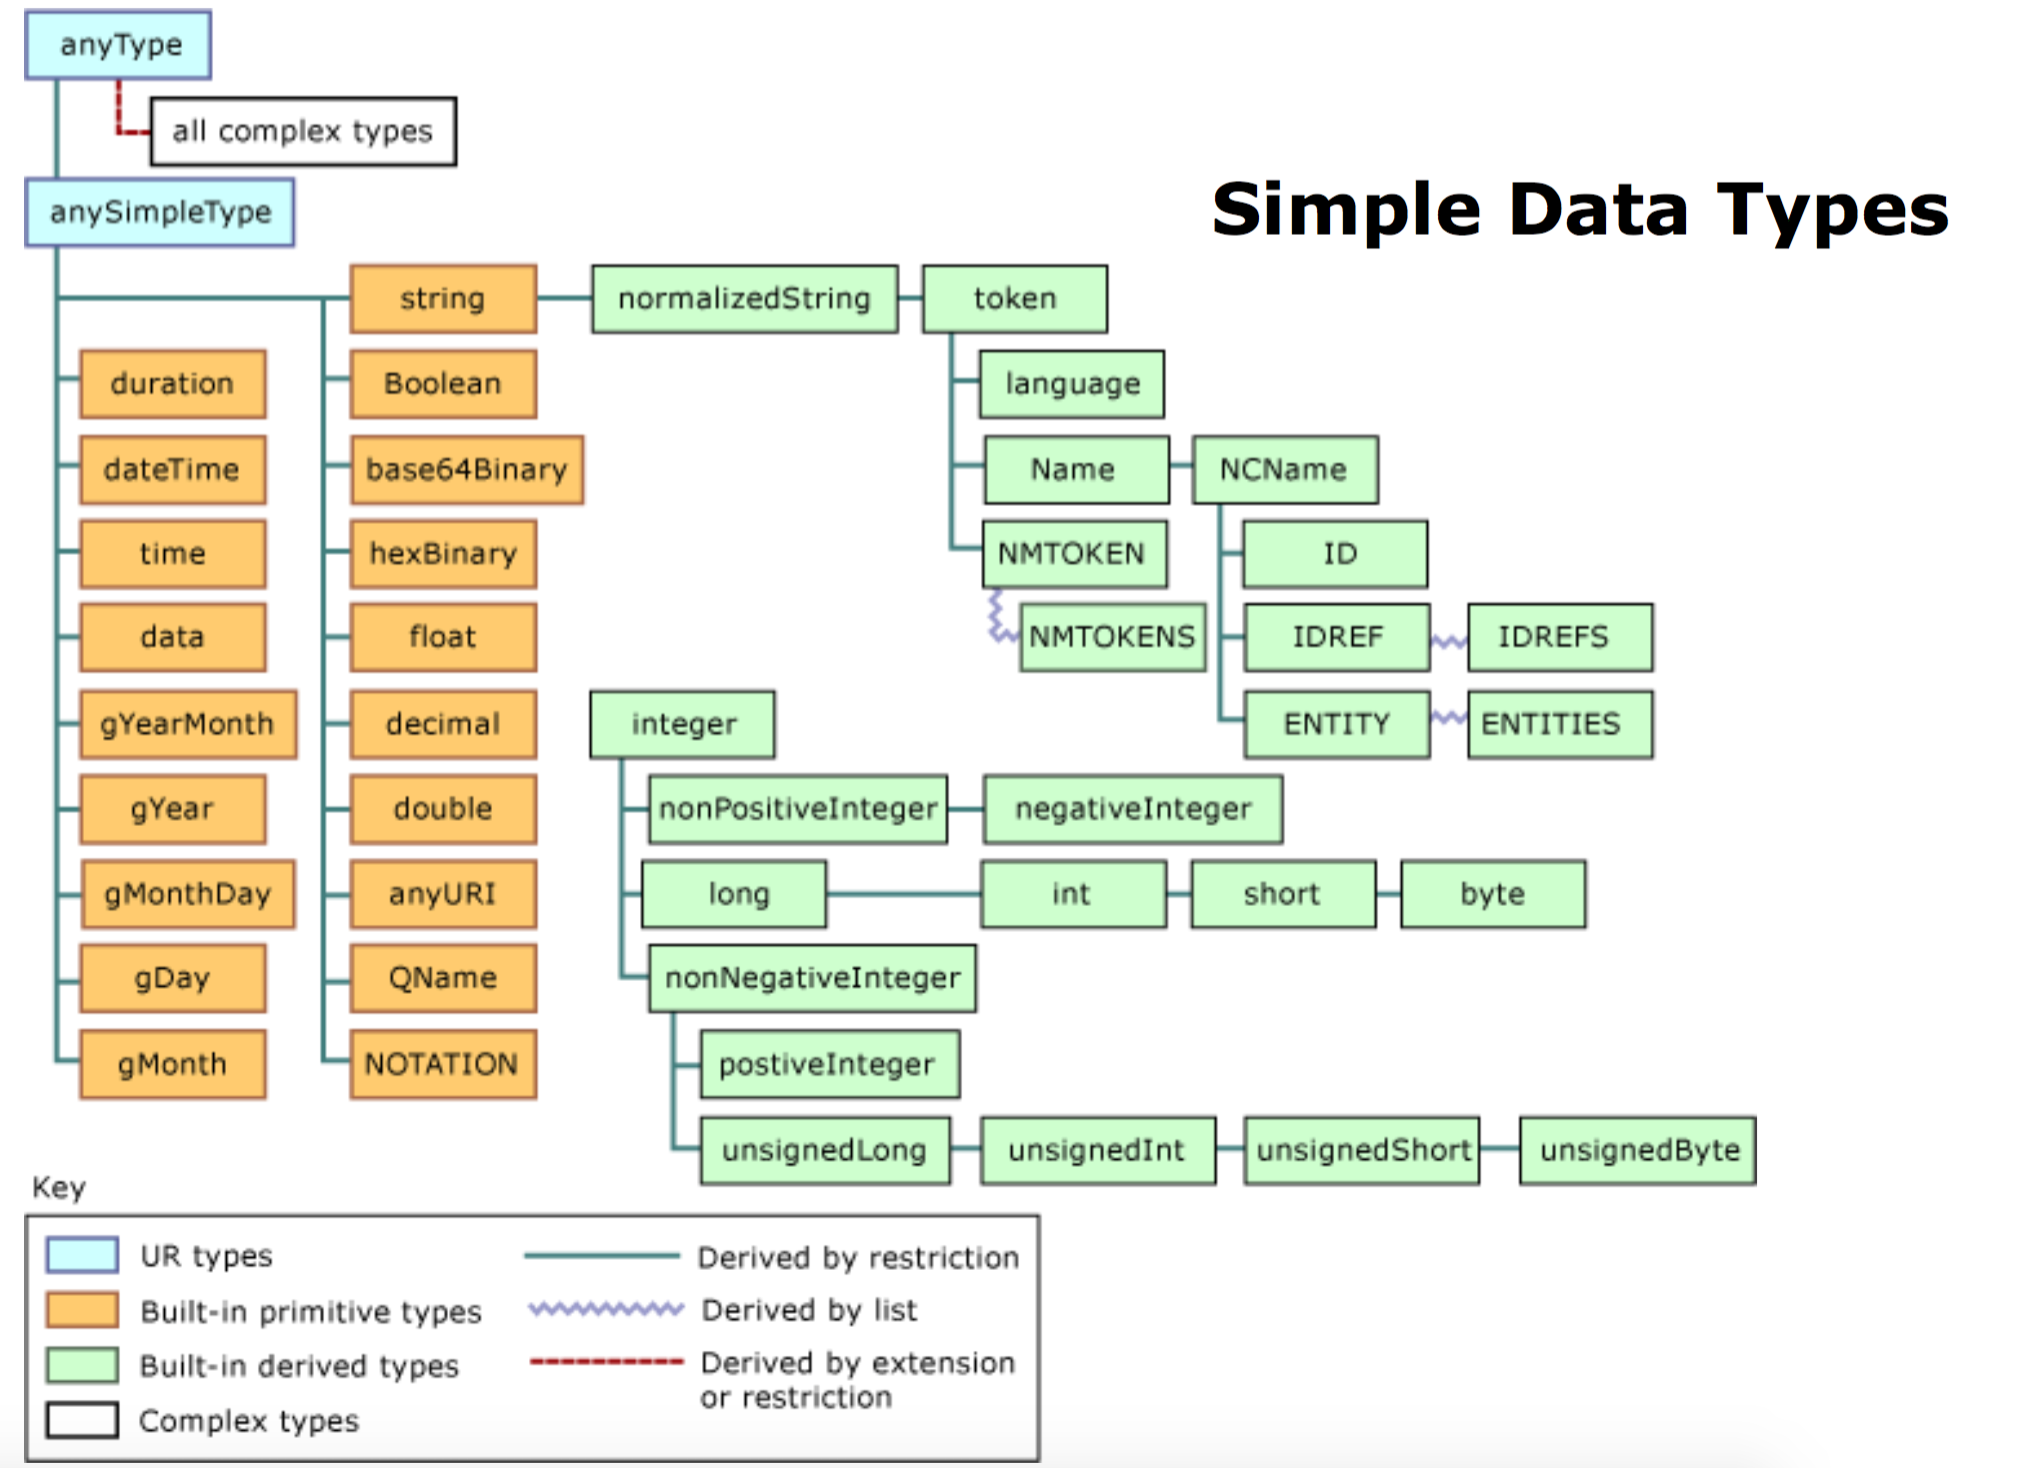
\includegraphics[width=\textwidth]{fig/SimpleDataTypes.png}
\end{figure}

\section{New Simple data Types by Restricition 1}
\begin{lstlisting}[language=XML, caption={Simple Elements}]
<xs:element name="population_under_15" type="percentType"/>
<xs:simpleType name="percentType"> 
	<xs:restriction base="xs:decimal">
		<xs:minInclusive value="0"/>
		<xs:maxInclusive value="100"/>
	</xs:restriction>
</xs:simpleType>
<xs:simpleType name="beer"> 
	<xs:restriction base="xs:string">
		<xs:enumeration value="Cardinal"/> 
		<xs:enumeration value="Lozaerner Bier"/> 
		<xs:enumeration value="Eichhof"/> 
		<xs:enumeration value="Boxer"/>
	</xs:restriction> 
</xs:simpleType>
\end{lstlisting}

\section{Constraints for Restrictions}
BIld hier einfügen

\section{Building Complex Types}
\begin{itemize}
\item Complex elements may contain sub-elements:
\begin{itemize}
\item <sequence> elements must appear in the given order,
\item <choice> if exactly one element is to be selected,
\item <all> elements can appear zero or one time in any order.
\end{itemize}
\item Complex elements may contain attributes.
\item Remember that an attribute is not a sub-element but an integral part. Therefore, even if an element only contains an attribute and nothing else, it is called complex type.
\end{itemize}

\section{Sequences with Local Definitions}

\begin{lstlisting}[language=XML, caption={Sequences with Local Definitions}]
<xs:element name="pets">
	<xs:complexType>
		<xs:sequence minOccurs="0" maxOccurs="unbounded">
			<xs:element name="dog" type="xs:string"/>
      		<xs:element name="cat" type="xs:string"/>
		</xs:sequence>
 	</xs:complexType>
</xs:element>
\end{lstlisting}
\red{\textbf{REIHENFOLGE MUSS SEIN: Zuerst alle Hunde, dann alle Katzen auflisten.}}

\section{Sequences with Global Definitions}
\begin{lstlisting}[language=XML, caption={Sequences with Global Definitions}]
<xs:element name="european_countries">
	<xs:complexType>
		<xs:sequence minOccurs="1" maxOccurs="unbounded">
			<xs:element ref="country"/>
		</xs:sequence>
	</xs:complexType>
</xs:element>
\end{lstlisting}
\begin{itemize}
\item At least one sub-element of type <country>.
\item If element <country> is defined globally it can be referenced.
\end{itemize}

\section{Choices}
Ist entweder-oder.
\begin{lstlisting}[language=XML, caption={Sequences with Global Definitions}]
<xs:element name="person">
	<xs:complexType>
		<xs:choice>
			<xs:element name="employee" type="xs:string"/>
			<xs:element name="player" type="xs:string"/>
		</xs:choice>
	</xs:complexType>
</xs:element>
\end{lstlisting}
\begin{itemize}
\item Casino employees are not supposed to play. A person in a casino must therefore either be an employee or a player (but not both).
\end{itemize}

\section{Sets}
\begin{lstlisting}[language=XML, caption={Sequences with Global Definitions}]
<xs:element name="country">
	<xs:complexType>
		<xs:all>
			<xs:element name="name" type="xs:string"/>
			<xs:element name="population" type="xs:positiveInteger"/>
		</xs:all> 
	</xs:complexType>
</xs:element>
\end{lstlisting}

The global definition of <country> could look like this. It must have exactly one element of type <name> and <population> in any order. We can change this to at most one as follows:

\begin{lstlisting}[language=XML, caption={Sequences with Global Definitions}]
<xs:element name="country">
	<xs:complexType>
		<xs:all minOccurs="0">
			<xs:element name="name" type="xs:string"/>
			<xs:element name="population" type="xs:positiveInteger"/>
		</xs:all>
	</xs:complexType>
</xs:element>
\end{lstlisting}


\section{Combining Complex Types}
Sequences and choices can contain elements that are complex types themselves. Sets (\code{<all>}) cannot. Also, sets cannot be combined
with other complex types as component of a complex type.
\begin{lstlisting}[language=XML, caption={Sequences with Global Definitions}]
<xs:complexType name="NameOrEmail">
	<xs:choice>
		<xs:element name="email" type="xs:string"/>
		<xs:sequence>
			<xs:element name="first" type="xs:string"/>
			<xs:element name="last" type="xs:string"/>
		</xs:sequence>
	</xs:choice>
</xs:complexType>
\end{lstlisting}

A global definition of a type (reusable by different elements) that can either be an email address or first and last name.\\
\red{\code{<all>}} cannot be used in this way !

\section{Simple Elements with Attributes}
What we want ...

\code{<product price="'2.00"'>Coffee in HSLU canteen</product>}\\
An element with simple (string) content and one (decimal) attribute. An element with attributes is a complex type (cf. slide 23).\\
\red{Do not confuse type with content !}
\begin{lstlisting}[language=XML, caption={Sequences with Global Definitions}]
<xs:element name="product">
	<xs:complexType>
		<xs:simpleContent>
			<xs:extension base="xs:string">
				<xs:attribute name="price" type="xs:decimal" />
			</xs:extension>
		</xs:simpleContent>
	</xs:complexType>
</xs:element>
\end{lstlisting}

\section{Attribute as Local Definition}
\begin{lstlisting}[language=XML, caption={Sequences with Global Definitions}]
<xs:element name="european_countries">
	<xs:complexType>
		<xs:sequence minOccurs="1" maxOccurs="unbounded"> 
			<xs:element ref="country"/>
		</xs:sequence>
		<xs:attribute name="year" type="xs:gYear" use="required"/>
	</xs:complexType>
</xs:element>
\end{lstlisting}
"`required"' bedeutet, dass das Attribut hier sein muss.
\begin{itemize}
\item Attribute values are restricted to simple types.
\item Attributes are optional by default unless use="'required"'
\item Attributes with default value:

\code{<xs:attribute name="language" type="xs:string" default="EN"/>}
\end{itemize}

\section{Attribute as Global Definition}
\textbf{Q}: Can I define and reference global attributes ?\\\\
\textbf{A}: Yes, but I do not recommend.\\

The XML Schema specification enforces that global elements or attributes must be qualified, i.e. belong to a namespace. For elements this is no problem. For qualified attributes, however, you cannot work with default namespaces in your instance document anymore.\\
Remember, even if an element belongs to a namespace, its attributes do not automatically belong to it. With qualified attributes you have to give them an explicit prefix. This is the same problem as with attributeFormDefault="qualified" in the root element.


\section{Additional Schema Features: Mixed Content}

\section{Additional Schema Features: Wildcards}
Eine Wildcard ist irgendeine 
\begin{lstlisting}[language=XML, caption={Sequences with Global Definitions}]
<xs:element name="catalogue"> 
	<xs:complexType>
		<xs:sequence>
			<xs:element name="Book" maxOccurs="unbounded">
				<xs:complexType>
					<xs:sequence>
						<xs:element name="Title" type="xs:string"/> 
						<xs:element name="Author" type="xs:string"/> 
						<xs:any namespace="##any" minOccurs="0"/>
					</xs:sequence>
				</xs:complexType>
			</xs:element>
		</xs:sequence>
	</xs:complexType>
</xs:element>
\end{lstlisting}

After \code{<Author>} \red{one} other well-formed XML element from any namespace \red{may} come. With the namespace attribute one may define from which namespace the unknown element is allowed to come in.

\section{Unique Particle Attribution}
\begin{lstlisting}[language=XML, caption={Sequences with Global Definitions}]
<xs:element name="catalogue"> 
	<xs:complexType>
		<xs:sequence>
			<xs:element name="Book" maxOccurs="unbounded">
				<xs:complexType>
					<xs:sequence>
						<xs:element name="Title" type="xs:string"/> 
						<xs:element name="Author" type="xs:string" minOccurs="0"/> 
						<xs:any namespace="##any" minOccurs="0"/>
					</xs:sequence>
				</xs:complexType>
			</xs:element>
		</xs:sequence>
	</xs:complexType>
</xs:element>
\end{lstlisting}
Es ist nun nicht klar, nach welchem Tag (Author oder \code{<any>}) der Code validiert wird $\rightarrow$ schwierig für Parser.

\section{Additional Schema Features: Lists}
In XML Schema:
\begin{lstlisting}[language=XML, caption={Sequences with Global Definitions}]
<xs:simpleType name="monthType"> 
	<xs:restriction base="xs:string">
		<xs:enumeration value="January"/> 
		<xs:enumeration value="February"/> 
		...
		<xs:enumeration value="December"/> 
	</xs:restriction>
</xs:simpleType>

<xs:element name="months">
	<xs:simpleType>
		<xs:list itemType="monthType"/>
	</xs:simpleType>
</xs:element>
\end{lstlisting}

\section{Additional Schema Features: Uniqueness 1}

\begin{lstlisting}[language=XML, caption={Sequences with Global Definitions}]
<xs:element name="bond_movies"> 
	<xs:complexType>
		<xs:sequence>
			<xs:element ref="movie" minOccurs="1" maxOccurs="unbounded"/>
		</xs:sequence>
		<xs:attribute name="month" type="monthType" use="required"/> 
		<xs:attribute name="year" type="xs:gYear" use="required"/>
	</xs:complexType>
	
	<xs:unique name="movieID"> 
		<xs:selector xpath="movie"/> 
		<xs:field xpath="@number"/>
	</xs:unique>
</xs:element>
\end{lstlisting}

\section{Additional Schema Features: Key References}
Referenzieren ist auch möglich. durch das \code{refer} Schlüsselwort wird sichergestellt, dass auf ein existierenden Key verwiesen wird.





\section{Control Questions A}
\begin{enumerate}
\item Unterschied Wohlgeformt und gültig.
\begin{itemize}
\item Wohlgeformt: Hat keine komischen Verschachtelungen USW
\item gültig: Entspricht einem Schema
\end{itemize}

\item Vorteile XML über DTD:
\begin{itemize}
\item Vererbung gibt es nicht in DTD
\item Keine Namespaces
\item Keine Enumerationen
\end{itemize}

\item Wann benötigt man ein XML Schema?\\
Spätestens wenn man ein XML Dokument benötigt (Schreibt oder liest).

\item Target Namespace\\
Man definiert einen Namen für seine eigene XML-Sprache.

\item Was bedeutet es, ein Element zu qualifizieren?\\
Der Target Namespace definiert den Namen seiner Sprache. Aber im XML kann man 

\item Was ist der Unterschied zwischen \code{<all>} und \code{<sequence>} und \code{<choice>}?\\
\code{<all>} muss alle enthalten ohne Reihefolge zu beachten, \code{<sequence>} beachtet reihenfolge und \code{<choice>} ist Mutual Exclusive (entweder oder).

\item Extension und Restriction\\
Extension macht zusätzliche Attribute möglich, Restriction bedeutet \textbf{nicht}, dass man Attribute löschen kann, aber man kann sie einschränken.

\item Automatische Typsubstitution von XML-Schema im vgl. zu Java:\\
Java kann man ein Interface definieren, vom Typ \code{Car} und dann kann man eine Klasse erstellen, die von \code{Car} ableitet und z.B. \code{BMW} heisst.
Erstellt man nun ein Array vom Typ \code{Car}, kann man ein Objekt vom Typ \code{BMW} direkt hineinspeichern.

Bei XML kann man das nicht, man verwendet dabei ein \code{type}-Attribut.
\end{enumerate}





\chapter{XSLT}
\section{Intro}
XSLT transforms documents from a source format to a target format. The source format must be an XML language, while the target format can be anything
However, in most cases the transformation is between XML languages. Typical target languages are XHTML, SVG or FO\\
XSLT is a declarative-functional programming language, i.e. you specify the result rather than how it is obtained.
\section{XSLT Basics and Conflicts}
XSLT-Stylesheets usually contains of templates. Each template specifies an XPath-like expression.
The following example has two different templates, one matching the root element ('/') ond one matching the movie nodes ('movie').
\begin{lstlisting}[language=XML]
<?xml version="1.0" ?>
<xsl:stylesheet version="1.0" xmlns:xsl="http://www.w3.org/1999/XSL/Transform">
  <xsl:template match="/">
    <html>
      <body>
<h1>This is a plain list of James Bond movie titles</h1> <ul>
          <xsl:apply-templates />
        </ul>
      </body>
</html>
  </xsl:template>
  <xsl:template match="movie">
<li>
      <xsl:value-of select="title"/>
</li>
  </xsl:template>
</xsl:stylesheet>
\end{lstlisting}
The XSLT-processort starts from the root of the source tree and finds the template which matches best. If more than one template matches,
a conflict resolution algorithm is called to determine the right template. Since the results vary from implementation to implementation,
ambigious templates should be avoided.\\
Rule:\\
 \green{\textbf{It is an error if this leaves more than one matching template rule.
An XSLT processor may signal the error; if it does not signal the error, it
must recover by choosing, from amongst the matching template rules that are left, the one that occurs last in the stylesheet.}}
\\
Rule:\\
\green{\textbf{More precise (restricting) templates are always executed first.}}

\section{Defining templates}
The first template should always start at the root element.
Each template has its context and all data requests are executed with respect to the context. Here, the context is \code{<movie>}
\begin{lstlisting}[language=XML]
<xsl:template match="movie">
  <li>
    <xsl:value-of select="title"/>
  </li>
</xsl:template>
\end{lstlisting}
Delegation to other template can be done using the \code{<apply-templates>} element which uses a select attribute
 to choose the nodes to process. The default value is the XPath expression node(). \\
 \begin{lstlisting}[language=XML]
<?xml version="1.0" ?>
<xsl:stylesheet version="1.0" xmlns:xsl="http://www.w3.org/1999/XSL/Transform">
<xsl:template match="/">
  <html>
  <h1>This is a plain list of James Bond movie titles</h1> <ul>
    <xsl:apply-templates select="bond_movies/movie/title" /> </ul>
  </html>
</xsl:template>
<xsl:template match="title">
  <li>
    <xsl:value-of select="text()"/>
  </li>
</xsl:template>
</xsl:stylesheet>
\end{lstlisting}
\section{Push vs. Pull processing}
Using a for-each loop as in the example below, is called pull-processing where using templates is called push-processing.
Elements can be pushed to a template or pulled to be used immediately. Templates are more like methods in other programming languages.
\begin{lstlisting}[language=XML]
<xsl:for-each select="bond_movies/movie">
    <li>
      <xsl:value-of select="title"/>
    </li>
</xsl:for-each>
\end{lstlisting}
Templates are better because:
\begin{itemize}
  \item Templates are more flexible and easier to maintain.
  \item Templates can be shared between stylesheets (see later).
  \item Templates can be overwritten (see later).
  \item Templates enable modular code.
\end{itemize}

\section {Conditional Logic}
There is an if statement (without else) which can be used as follows:
\begin{lstlisting}[language=XML]
<xsl:template match="movie">
  <xsl:if test="duration &gt; 130">
    <li style="color:red"> <xsl:value-of select="title"/>
    </li>
  </xsl:if>
  <xsl:if test="duration &lt;= 130">
    <li>
      <xsl:value-of select="title"/>
    </li>
  </xsl:if>
</xsl:template>
\end{lstlisting}
And there's the choose-statement for multiple conditions:
\begin{lstlisting}[language=XML]
<xsl:template match="movie">
  <xsl:choose>
    <xsl:when test="duration &gt; 140">
      <li style="color:red"><xsl:value-of select="title"/></li>
    </xsl:when>
    <xsl:when test="duration &gt; 120">
      <li style="color:orange"><xsl:value-of select="title"/></li>
    </xsl:when>
    <xsl:otherwise>
      <li style="color:green"><xsl:value-of select="title"/></li>
    </xsl:otherwise>
  </xsl:choose>
</xsl:template>
\end{lstlisting}

\section{Producing XHTML}
XHTML requires a default namespace in the <html> element. This can be achieved by adding the XHTML namespace as
default namespace to the XSLT file. It will then be carried over to the output document. Like this:
\begin{lstlisting}[language=XML]
<xsl:stylesheet version="1.0" xmlns:xsl="http://www.w3.org/1999/XSL/Transform" xmlns="http://www.w3.org/1999/xhtml" >
\end{lstlisting}
Because the XHTML-Namespace has to be the default namespace, all the other namespaces have to be imported using prefixes.\\
XHTML is still validated against DTDs, so we may want to refer to the right DTD in our output document. Like this:
\begin{lstlisting}[language=XML]
<xsl:output doctype-public="-//W3C//DTD XHTML 1.0 Strict//EN" doctype-system="http://www.w3.org/TR/xhtml1/DTD/xhtml1-strict.dtd" />
\end{lstlisting}


\section{Sorting elements}
<sort> can be used as a child of <apply-templates> or <for-each>.
It has three attributes: select, data-type and order. The possible values for order are ascending or descending. Here's an example:
\begin{lstlisting}[language=XML]
<xsl:apply-templates select="movie[starts-with(bond/text(), 'Pierce')]">
  <xsl:sort select="bond_girl" data-type="text" order="descending"/>
</xsl:apply-templates>
\end{lstlisting}

\section{Named templates}
Instead of (or in addition to) using the match attribute we can call templates by name. This has the following advantages:\\
1. We can split up large templates and reuse elsewhere\\
2. We can pass parameters to the template. Inside the template,
parameter values are accessed by \code{\$para\_name} like this:
\begin{lstlisting}[language=XML]
<xsl:template name="header">
  <xsl:param name="color" />
  <tr style="background-color:{$color}">
      <th>Title</th>
      <th>Bond Actor</th>
      <th>Bond Girl</th>
      <th>Producer</th>
      <th>Year</th>
      <th>Length</th>
  </tr>
</xsl:template>
\end{lstlisting}
And then be called using the name with a parameter: (name of the parameters are global)
\begin{lstlisting}[language=XML]
<xsl:call-template name="header">
  <xsl:with-param name="color">#990066</xsl:with-param>
</xsl:call-template>
\end{lstlisting}
\red{\textbf{Use named templates if parameter values remain constant, use matching when you need to use data out of the XML.}}

\section{More XSLT features}
\begin{itemize}
  \item Variables can be defined as follows:\\
  \code{<xsl:variable name="version" >1.0beta</xsl:variable>}\\
  However, variables can be initialized only once in their lifetime.
  \item \code{<copy-of select="path" />}\\ Copies content from the source to the output tree,
   i.e. it copies the specified node with its children and attributes.
   This is very handy if you want to transform a document into a modified form of itself.
   \item \code{<import href="path" />}\\ Thi can be used to include another stylesheet by just copy- pasting its content to the current file.
    This enables to build modules of reusable code. In case of conflicts, the imported templates obtain lower priority.
    \item Getting Content from other XML Files:\\
    We can access information in other XML files using the function document(url). The specification allows any URL but processors
generally support only paths (see below), HTTP and HTTPS.
In bond\_movies.xml each movie has an attribute id. Imagine now another file bond\_movies\_media.xml that stores poster images for each movie referenced by ID.
We can get the poster for ID \_02 as follows:
\begin{lstlisting}[language=XML]
  <img src="{document('bond_movies_media.xml')/ bond_movies/movie[@number='_02']/poster/@href}"
  alt="{document('bond_movies_media.xml')/ bond_movies/movie[@number='_02']/title}"/>
\end{lstlisting}
\end{itemize}


\section{XSLT Bootcamp Übung}
\input{BootCamp/XSLT/xslt_bootcamp}

\chapter{XQueries}
\section{Native XML Databases}
A Native XML Database is a computer system that holds the following properties:
\begin{itemize}
  \item It is a database, i.e. a software component integrating both (1) a structured collection of data and (2) access programs to define, manipulate and query that data
  \item Data are stored in documents. It is therefore a special kind of document store.
  \item Data in the documents comply with the XML standard.
  \item XML technologies such as XPath, Xquery or XSL/T can be applied for querying and manipulating data in the database.
\end{itemize}


\section{XML-DB vs SQL-DB}

\begin{table}[htbp]
\centering
\caption{Comparison XML vs. SQL}
\begin{tabular}{ll}
\textbf{XML DB}         & \textbf{SQL DB}        \\ \cline{1-2}
\multicolumn{1}{|l|}{Hierarchical} & \multicolumn{1}{l|}{Relational} \\ \cline{1-2}
\multicolumn{1}{|l|}{Fast access of nested structures} & \multicolumn{1}{l|}{Slow access of nested structures (join)} \\ \cline{1-2}
\multicolumn{1}{|l|}{Works well for aggregating data (1:n)} & \multicolumn{1}{l|}{Works well for interrelated data (n:m) } \\ \cline{1-2}
\multicolumn{1}{|l|}{Working with files and XML-documents directly } & \multicolumn{1}{l|}{Working with abstract tables and tuples} \\ \cline{1-2}
\multicolumn{1}{|l|}{Focus on structure (XSD, DTD)} & \multicolumn{1}{l|}{Focus on consistency (ACID)} \\ \cline{1-2}
\multicolumn{1}{|l|}{Ideal for web applications} & \multicolumn{1}{l|}{Ideal for banking applications} \\ \cline{1-2}

\end{tabular}
\end{table}

\section{XQuery}
XQuery is a language for searching and manipulating data in XML Trees (XDM)\\
XQuery expressions can access data over multiple documents and databases, and extract results very efficiently.\\
XQuery is a FLWOR-expression (pronounced flower), with main syntax elements:\\FOR-LET-WHERE-ORDER-RETURN\\
\\
XQuery is a true superset of XPath, meaning that every single valid
XPath expression is also a valid XQuery expression.\\
Xquery is an extension to Xpath, allowing for nested loops with SQL- like elements such as where statements and order-by clauses.\\
XPath lets you find XML elements by path expressions.\\
XQuery, however, adds a couple of additional powerful constructs that allow you to do much more and let you manipulate or construct entire XML documents on the fly.\\
  => return clause is essential for this feature, where new and arbitrary XML can be added and combined with results from the query

\section{FLWOR and examples}

\begin{itemize}
  \item for: define variables (start name with \$) as FLWOR-Expression
(normally just an Xpath-expression)
  \item let: new variables for some (aggregated) subsets of the for-variables
  \item where: some restrictions on/ between the for-variables and XPath- expressions starting from the for-variables
  \item order: some variable with Xpath-expression (must be a singleton!)
  \item return: a valid XML-structure constructed of constants and Xpath- expressions starting from variables. If constants and expressions are mixed: expressions must be set in curly brackets ({}) – otherwise they are not evaluated, but also taken as (constant) strings!!
\end{itemize}
Beispiel 1:
\begin{lstlisting}[language=XML]
for $v in //Vorlesung
let $orderVar := $v/SWS
where $v/../..[Name="Sokrates"]
order by $orderVar descending
return <Vorlesung>{$v/Titel}{$v/SWS}</Vorlesung>
\end{lstlisting}
returns:
\begin{lstlisting}[language=XML]
<Vorlesung><Titel>Ethik</Titel> <SWS>4</SWS></Vorlesung>
<Vorlesung><Titel>Logik</Titel><SWS>4</SWS></Vorlesung>
<Vorlesung><Titel>Maeeutik</Titel><SWS>2</SWS></Vorlesung>
\end{lstlisting}


\chapter{Formatting Objects}



\section{Control Questions}
\begin{enumerate}
\item Purpose of XSL-FO\\
Daten in XML zu einem printbaren Medium konvertieren. Mit einem Prozessor kann es dann umgewandelt werden in z.B. PDF.
\item 2-Phasen Modell\\
1. Phase ist XSL-Transformation, 2.Phase ist FO-Transfromation
\item Allgemeiner Aufbau\\
Normalerweise 2 Sections: 1. definiert Layout der Seite, 2. definiert Inhalt in Blöcken und in welchem Flow er sich befindet. Der Flow speist dann die Seite.
\item 
\end{enumerate}




\chapter{SVG}
\section{Theory summary}
SVG is an XML format to define vector graphics. But you can also have the best of both worlds, SVG allows to embed bitmap images.\\
SVG is widely used to define pictures and animations. It recently gained importance when it became part of the Open Web Platform\\
introduced with HTML 5.
Webbrowsers display SVG natively.\\
SVG graphics are most often created using graphical editors such as Inkscape for example. You can even create SVG graphics in your\\
browser – try here.
Alternatively, we may directly manipulate an SVG DOM tree from our programs or, as in this course, produce SVG using XSLT.\\
\section{Control Questions}

\begin{enumerate}
\item Explain the difference between a bitmap and a vector image.\\
\textit{bitmap wird f\"{u}r Fotos verwendet $\rightarrow$ Ansammlung von Pixel und vector image f\"{u}r Grafiken und Diagramme, sie setzen sich aus einer Vektroren Beschreibung zusammen.}

\item Name advantages and disadvantages of each format.\\
\textit{Vektor ist kleiner und Skalierbar da es anhand der Beschreibung neu gezeichnet wird, Bitmap hat Fotografische Qualität, leichter Portierbar, weniger Träge von Maleware}

\item Explain how SVG paths work.\\
\textit{Eine Sequenz von Knoten mit Verbindungslinien dazwischen mit relativen und Absoluten Pfaden (grosse und Kleine buchstaben)}

\item What is the purpose and practical importance of XLink ?\\
\textit{wird nur in SVG, MathML ben\"{o}tigt f\"{u}r verlinkung}


\item Where is XLink used in SVG ?\\
\textit{Um definierte Grafiken zu referenzieren und an anderen orten wieder zu verwenden.}

\item Name different methods of how SVG documents are created and manipulated in practice.\\
\textit{Fragen k\"{o}nnne selber geparst werden}

\item How can we equip SVG graphics with animations ?\\
\textit{smil}
\end{enumerate}

\end{enumerate}



\chapter{Processing XML with Java \& Stuff}
\section{Control Question}
\begin{enumerate}
\item XML documents can be processed sequentially or by creating an in-memory representation. Name advantages, disadvantages and a framework implementation of each variant\\

\begin{tabular}{|p{0.12\linewidth}|p{0.3\linewidth}|p{0.3\linewidth}|p{0.12\linewidth}|}
\hline
Technology & Advantages & Disadvantages & Framework\\
\hline
Sequential & Wenn Zeilennummer ausgegeben werden muss, Memorysparend, bei sehr grossen Files & Schwierig zu programmieren, nicht intuitiv & SAX\\
\hline
In-Memory & Gute OO-Unterstützung, XPath kann verwendet werden & Braucht ca. 4-fachen Speicher des Dokuments & LINQ, JDOM\\
\hline
\end{tabular}
\item What is the different between pull and push processing ?\\
\begin{itemize}
\item push: Eventbasiert, Framework pusht in eigenen Eventhandler
\item pull: Man "`holt"' sich die Daten aus dem Dokument, durchläuft es selbständig.
\end{itemize}
\item Explain the steps for processing an XML document with SAX.
\begin{enumerate}
\item Create a parser
\item Give DefaultHandler extension to parser
\item Start reader on XMLFile
\end{enumerate}
\item What is the difference between DOM, JDOM and XDOM ?\\
DOM: Ursprüngliche Implementierung\\
JDOM: Java Implementation, hat NICHTS mit DOM zu tun, ausser, dass es auch eine In-Memory Darstellung ist.\\
XDOM: .NET Implementation
\item Explain the steps for processing an XML document with JDOM.\\
\begin{enumerate}
\item XML Element in Parser füttern
\item Parser spuckt Dokument aus
\item Dokument kann traversiert werden
\end{enumerate}
\item Explain the steps for invoking an XSL transformation from Java.\\
\begin{enumerate}
\item XML Dok laden
\item XSL Dok laden
\item spezifizieren, wohin das Resultatdokument geschrieben wird.
\end{enumerate}
\end{enumerate}




\chapter{Pruefungsinfos}
\section{Aufteilung}
\[
\frac{50 \textnormal{ Punkte}}{5 \times 10 \textnormal{ Punkte}}
\]

\[
\underbrace{f(net)=\begin{cases}
0 & \text{für } net_j \le -n \\
\frac{net_j}{2n} + \frac{1}{2} & \text{für } -n \le net_j \le n \\
1 &\text{für } net_j \ge n 
\end{cases}}_{a)} \hspace{3cm}
\underbrace{f(net)=\frac{1}{1+e^{-anet}}}_{b)}
\]

\begin{itemize}
\item XPATH mit Bootcamp
\item XML Schema mit Bootcamp
\item XSLT + XHTML (Tabelle oder Bullet List) mit Bootcamp
\item XQuery
\item Theory
\end{itemize}


\end{document}